% =====================================================================
%  CS 360 -- Sprint 2 Project Documentation
%  Codey: A Gamified Computer Science Study App
%  Build:  tectonic Sprint2_Documentation.tex   (or pdflatex, run twice)
% =====================================================================
\documentclass[12pt,letterpaper]{article}

% ---------- Page layout & typography --------------------------------
\usepackage[margin=1in]{geometry}
\usepackage[T1]{fontenc}
\usepackage[utf8]{inputenc}
\usepackage{newtxtext,newtxmath}
\usepackage{setspace}
\doublespacing
\usepackage{microtype}
\usepackage{parskip}
\usepackage{xcolor}
\usepackage{etoolbox}
\usepackage{enumitem}
\setlist{nosep}
\emergencystretch=3em

% ---------- Tables ----------------------------------------------------
\usepackage{array}
\usepackage{booktabs}
\usepackage{xltabular}
\newcolumntype{L}[1]{>{\raggedright\arraybackslash}p{#1}}
\newcolumntype{Y}{>{\raggedright\arraybackslash}X}

% Tables and figures are single-spaced so they stay readable.
\AtBeginEnvironment{table}{\singlespacing\footnotesize\renewcommand{\arraystretch}{1.25}}
\AtBeginEnvironment{xltabular}{\singlespacing\footnotesize\renewcommand{\arraystretch}{1.25}}
\AtBeginEnvironment{figure}{\singlespacing}

% ---------- Captions / references -------------------------------------
\usepackage[font=small,labelfont=bf,skip=6pt]{caption}
\usepackage{float}
\usepackage[section]{placeins}
\usepackage{graphicx}
\graphicspath{{figures/}}
\usepackage[hidelinks]{hyperref}

% ---------- Diagrams --------------------------------------------------
\usepackage{tikz}
\usetikzlibrary{positioning,arrows.meta,shapes.geometric,shapes.multipart,
                fit,backgrounds,calc}
\usepackage{pgfgantt}

\newcommand{\st}[1]{\guillemotleft#1\guillemotright}   % <<stereotype>>
\newcommand{\ctitle}[1]{{\centering #1\par}}   % centred class-name compartment
\newcommand{\priv}{\ensuremath{-}}                       % UML private
% UML required-interface socket on ball #1, opening toward angle #2 (90 = up).
\newcommand{\sock}[2]{\draw[line width=0.6pt] ([shift={(#2-90:0.24)}]#1.center)
  arc[start angle=#2-90, delta angle=180, radius=0.24];}

\tikzset{
  % UML class box: #1 = colour, #2 = width
  cls/.style n args={2}{draw=#1!70!black, line width=0.6pt,
      rectangle split, rectangle split parts=3,
      rectangle split part fill={#1!22,#1!6,#1!6},
      text width=#2, font=\sffamily\scriptsize, inner sep=3pt},
  % Arrow styles (UML 2.5 notation)
  assoc/.style   ={line width=0.6pt, -{Straight Barb[length=2mm]}},
  dep/.style     ={line width=0.6pt, dashed, -{Straight Barb[length=2mm]}},
  realize/.style ={line width=0.6pt, dashed, -{Triangle[open,length=2.6mm,width=2.6mm]}},
  compo/.style   ={line width=0.6pt, {Diamond[length=3.2mm,width=2.2mm]}-},
  aggr/.style    ={line width=0.6pt, {Diamond[open,length=3.2mm,width=2.2mm]}-},
  lbl/.style     ={font=\sffamily\scriptsize, fill=white, inner sep=1.5pt},
  glbl/.style    ={font=\sffamily\scriptsize, fill=gray!22, inner sep=2pt, align=center},
  % Use-case elements
  usecase/.style ={ellipse, draw, line width=0.6pt, fill=white, align=center,
      text width=2.3cm, inner sep=0pt, minimum height=1.05cm,
      execute at begin node=\hyphenpenalty 10000\relax, font=\sffamily\scriptsize},
  store/.style   ={cylinder, shape border rotate=90, aspect=0.25, draw, line width=0.6pt,
      fill=white, minimum height=1.45cm, minimum width=2.1cm, align=center,
      font=\sffamily\scriptsize},
  % State-machine elements
  state/.style   ={rectangle, rounded corners=3pt, draw, line width=0.7pt, fill=white,
      minimum width=2.6cm, minimum height=0.75cm, font=\sffamily\small},
  trans/.style   ={line width=0.6pt, -{Stealth[length=2.2mm]}, rounded corners=2pt},
  % Component / deployment elements
  comp/.style    ={rectangle, draw, line width=0.6pt, fill=white, align=center,
      text width=2.9cm, minimum height=1.25cm, font=\sffamily\scriptsize},
  ball/.style    ={circle, draw, line width=0.6pt, fill=white, minimum size=2.8mm, inner sep=0pt},
  artifact/.style={rectangle, draw, line width=0.6pt, fill=white, align=center,
      text width=2.5cm, minimum height=1.0cm, font=\sffamily\scriptsize},
}

% Stick-figure actor
\tikzset{stickman/.pic={
  \draw[line width=0.7pt] (0,0.42) circle (0.13);
  \draw[line width=0.7pt] (0,0.29) -- (0,-0.08)
        (-0.22,0.17) -- (0.22,0.17)
        (0,-0.08) -- (-0.18,-0.42)
        (0,-0.08) -- (0.18,-0.42);
}}

% Small UML component icon in the top-right corner of node #1
\newcommand{\compicon}[1]{%
  \draw[line width=0.4pt,fill=white] ([shift={(-0.42,-0.12)}]#1.north east) rectangle ++(0.28,-0.34);
  \draw[line width=0.4pt,fill=white] ([shift={(-0.48,-0.19)}]#1.north east) rectangle ++(0.12,-0.07);
  \draw[line width=0.4pt,fill=white] ([shift={(-0.48,-0.32)}]#1.north east) rectangle ++(0.12,-0.07);
}

% 3-D box faces for a UML deployment node #1 with colour #2
\newcommand{\nodebox}[2]{%
  \draw[line width=0.6pt,fill=#2!35] (#1.north west) -- ++(0.35,0.35)
      -- ([shift={(0.35,0.35)}]#1.north east) -- (#1.north east) -- cycle;
  \draw[line width=0.6pt,fill=#2!45] (#1.north east) -- ++(0.35,0.35)
      -- ([shift={(0.35,0.35)}]#1.south east) -- (#1.south east) -- cycle;
}

% ---------- Section formatting ----------------------------------------
\usepackage{sectsty}
\allsectionsfont{\raggedright}
\setcounter{secnumdepth}{2}
\setcounter{tocdepth}{2}

\begin{document}

% =====================================================================
%  COVER PAGE
% =====================================================================
\begin{titlepage}
\begin{singlespace}
\centering
\vspace*{1.2in}
{\LARGE\bfseries Codey\par}
\vspace{0.25cm}
{\Large Gamified Computer Science Study App\par}
\vspace{1.2cm}
{\large CS 360: Software Engineering I\par}
\vspace{0.3cm}
{\large Sprint 2 Project Documentation\par}
\vspace{0.3cm}
{\large Sprint Period: September 13 -- October 3, 2026\par}
\vspace{0.3cm}
{\large Date Submitted: October 1, 2026\par}
\vspace{1.6cm}
{\large\bfseries Team Members\par}
\vspace{0.4cm}
\begin{tabular}{lll}
\toprule
\textbf{Name} & \textbf{Role} & \textbf{Email} \\
\midrule
Raaj Banga        & Project Manager            & manraaj.banga277@topper.wku.edu \\
Arnav Bawankule   & Backend \& Systems Lead    & arnav.bawankule838@topper.wku.edu \\
Elnad Salcinovic  & iOS UI/UX \& QA Lead       & elnad.salcinovic250@topper.wku.edu \\
\bottomrule
\end{tabular}
\vfill
{\large Client: Dr.\ Galloway\par}
\vspace{0.5in}
\end{singlespace}
\end{titlepage}

% =====================================================================
%  TABLE OF CONTENTS
% =====================================================================
\pagenumbering{arabic}
\setcounter{page}{2}
\begin{singlespace}
\tableofcontents
\clearpage
\listoffigures
\listoftables
\end{singlespace}
\clearpage

% =====================================================================
\section{Project Overview and Scope (Updated for Sprint 2)}
% =====================================================================

\subsection{Project Overview}
Codey is a native iOS study application for computer science that combines the game
mechanics of Duolingo with the flashcard-based study model of Quizlet. It is intended
for undergraduate computer science students and students in introductory programming
courses. The client is Dr.\ Galloway. Codey is developed as a course project and is
demonstrated by the team from Xcode. It will not be distributed through the App Store.

The planned product comprises six feature areas:
\begin{itemize}
  \item \textbf{Flashcard decks.} Students build their own decks in the app, supplemented by developer-authored starter
        decks for each topic, and may attach
        syntax-highlighted code examples to individual cards. Decks remain available
        offline and are synchronized across devices.
  \item \textbf{Adaptive practice.} Questions in each topic are grouped into Easy,
        Medium, and Hard tiers. Mastered questions are retired from practice, and
        higher tiers unlock as the student progresses.
  \item \textbf{Gamification.} Students earn experience points (XP), levels, daily
        streaks, and badges.
  \item \textbf{Progress analytics.} The app tracks accuracy by topic and generates
        personalized study plans from that data.
  \item \textbf{Code-completion exercises.} Students fill in the missing parts of
        partially written code snippets in an in-app editor, and each answer is checked
        against automated test cases.
  \item \textbf{Leaderboards and weekly challenges.} Students compete within a class,
        club, or friends list.
\end{itemize}
Section~\ref{sec:reqs} specifies the requirements for each feature area.

\begin{table}[H]
\centering
\caption{Team roles and responsibilities}
\label{tab:team}
\begin{tabularx}{\textwidth}{@{}L{3.1cm} L{3.3cm} Y@{}}
\toprule
\textbf{Member} & \textbf{Role} & \textbf{Responsibilities} \\
\midrule
Raaj Banga & Project Manager (Sprints 1 and 2) & Sprint planning, backlog and schedule, deliverable coordination, client liaison, sprint documentation. \\
Arnav Bawankule & Backend \& Systems Lead & Database architecture, Supabase configuration, cloud sync, encryption standards, exercise validation. \\
Elnad Salcinovic & iOS UI/UX \& QA Lead & SwiftUI components, offline caching (SwiftData), responsive layouts, test harness and QA. \\
\bottomrule
\end{tabularx}
\end{table}

\subsection{Changes Since Sprint 1}
Sprint 2 advanced the project from feasibility and planning to architecture, design,
and implementation of the core study and synchronization features. The principal
changes are:
\begin{itemize}
  \item \textbf{Backend selection.} Supabase (PostgreSQL, PostgREST, and GoTrue
        authentication) was selected as the cloud backend, with Google Sign-In as the
        authentication method.
  \item \textbf{UML modeling.} Use case, sequence, state, class, component, and
        deployment models were produced for the deck-creation and synchronization
        workflow, and kept consistent with the implementation.
  \item \textbf{Design patterns.} One Gang of Four pattern was adopted from each
        category: Factory (creational), State (behavioral), and Fa\c{c}ade (structural).
  \item \textbf{Requirements revision.} The requirements were rewritten as 49 atomic
        functional requirements and 20 non-functional requirements.
  \item \textbf{Decks, study, and quizzes.} The deck builder (a card pager with
        Markdown text and an optional code snippet), twelve tier-tagged starter decks,
        a study mode with a 3D card flip and swipe-to-rate, and topic quizzes are
        complete (FR-05 to FR-21).
  \item \textbf{Adaptive practice and gamification.} Question retirement, the
        70\% tier unlocks, review returns, restricted practice, XP, and levels are
        implemented (FR-22 to FR-31). XP includes a capped streak bonus (FR-30).
  \item \textbf{Accounts and synchronization.} Google Sign-In, the Supabase schema
        with Row Level Security, the sync queue, the push/pull sync engine, and the
        additive conflict merge are implemented behind \texttt{BackendFacade}
        (FR-01 to FR-03, FR-44 to FR-48). Sign-in is optional; the app works fully
        as a guest.
  \item \textbf{User interface.} The app is organized around a Home hub that shows
        level, XP, and per-topic accuracy (FR-36, FR-37), with a three-tab Liquid Glass
        tab bar, a profile sheet, and first-launch onboarding, on a token-based design
        system (Section~\ref{sec:ui}).
  \item \textbf{Third-party libraries.} Textual renders card Markdown and code, and
        Runestone with Tree-sitter grammars provides the code editor (NFR-15,
        risk R12).
  \item \textbf{Platform.} The minimum deployment target was raised to iOS 26
        (NFR-03) to use the system Liquid Glass and tab-bar APIs.
\end{itemize}

\subsection{Scope}
Table~\ref{tab:scope} defines the project scope. Personalized study plans,
leaderboards, and weekly challenges are client-mandated but were omitted from the
Sprint 1 scope; they have been added in this revision. Table~\ref{tab:moscow}
prioritizes features using the MoSCoW method. Features in the Could Have category are
built last and are the first candidates for de-scoping if the schedule slips
(Section~\ref{sec:risks}). Any change to scope requires client approval.

The client-mandated coding challenges are scoped as code-completion
(fill-in-the-blank) exercises. Each answer is validated by comparison with accepted
solutions, so no code is compiled or executed on the device. Open-ended,
LeetCode-style problems that require running arbitrary code are a stretch goal. The
team will pursue them only if a working code-execution prototype exists by the end of
Sprint 3 (risk R1).

\begin{table}[H]
\centering
\caption{In-scope and out-of-scope features (updated for Sprint 2)}
\label{tab:scope}
\begin{tabularx}{\textwidth}{@{}Y Y@{}}
\toprule
\textbf{In Scope (will build)} & \textbf{Out of Scope (will not build)} \\
\midrule
User-built flashcard decks with optional code snippets, plus bundled starter decks & Multi-language (localization) support \\
Adaptive practice with Easy/Medium/Hard question tiers that rotate as questions are mastered & Real-time multiplayer (leaderboards and weekly challenges are asynchronous) \\
XP, levels, streaks, and badges & Advertisements and in-app purchases \\
Per-topic progress analytics and personalized study plans & Direct messaging between users \\
Code-completion (fill-in-the-blank) exercises with automated validation & Full IDE functionality \\
Leaderboards and weekly challenges (class, club, or friends list) & Importing decks from files (user decks are built in the app; starter decks are bundled) \\
Offline data caching and cloud sync & App Store distribution (demonstrated from Xcode only) \\
Secure data handling (encryption and row-level access control) & Paid third-party services \\
\bottomrule
\end{tabularx}
\end{table}

\begin{table}[H]
\centering
\caption{Feature prioritization (MoSCoW)}
\label{tab:moscow}
\begin{tabularx}{\textwidth}{@{}Y Y Y@{}}
\toprule
\textbf{Must Have} & \textbf{Should Have} & \textbf{Could Have} \\
\midrule
User-created flashcards & XP and leveling system & Daily streaks \\
Working SwiftUI interface & Cloud data sync & Leaderboards \\
Easy/Medium/Hard difficulty & Dark/Light mode & Personalized study plan \\
Adaptive tier rotation (client mandate) & Performance analytics & Customized profile \\
Navigation that adapts to all supported iPhone screen sizes (NFR-10) & Starter decks & Code-completion exercises \\
Stable operation (no crashes during scripted test sessions) & & Weekly challenges \\
 & & Badges \\
 & & Open-ended coding problems (stretch) \\
\bottomrule
\end{tabularx}
\end{table}

% =====================================================================
\section{Requirements (Updated for Sprint 2)}\label{sec:reqs}
% =====================================================================
Requirements are written in accordance with ISO/IEC/IEEE 29148:2018. Each
requirement is a single, verifiable ``shall'' statement with a unique identifier that
is referenced in the traceability matrices (Section~\ref{sec:trace}). \emph{Priority}
follows the MoSCoW scale in Table~\ref{tab:moscow}. \emph{Source} indicates whether
the requirement originates from the client's mandatory list or from the team.
\emph{Status} reflects progress at the time of submission: \emph{Implemented} (built,
covered by passing tests, and merged), \emph{In progress} (partly built), or
\emph{Planned} (scheduled for a later sprint). Sprint 1 requirements that specified
more than one behavior were decomposed in Sprint 2, and identifiers were reassigned
accordingly.

\subsection{Functional Requirements}

\begin{xltabular}{\textwidth}{@{}l Y l l l@{}}
\caption{Functional requirements}\label{tab:fr}\\
\toprule
\textbf{ID} & \textbf{Requirement} & \textbf{Priority} & \textbf{Source} & \textbf{Status} \\
\midrule
\endfirsthead
\multicolumn{5}{@{}l}{\small\itshape Table \thetable\ continued} \\
\toprule
\textbf{ID} & \textbf{Requirement} & \textbf{Priority} & \textbf{Source} & \textbf{Status} \\
\midrule
\endhead
\bottomrule
\endfoot
\multicolumn{5}{@{}l}{\textit{Account and authentication}} \\
FR-01 & The app shall allow a user to sign in with a Google account through Supabase Auth. & Must & Team & Implemented \\
FR-02 & The app shall store the authenticated session token in the iOS Keychain. & Must & Client & Implemented \\
FR-03 & The app shall allow a signed-in user to sign out, which deletes the stored session token from the Keychain and lets the user choose whether to keep or remove that account's decks on the device. & Must & Team & Implemented \\
FR-04 & The app shall allow a user to set a display name of 1--30 characters and choose an avatar from a predefined set. & Could & Team & Planned \\
\multicolumn{5}{@{}l}{\textit{Decks and flashcards}} \\
FR-05 & The app shall allow a user to create a flashcard deck with a title of 1--60 characters and a topic category chosen from a predefined list. & Must & Team & Implemented \\
FR-06 & The app shall allow a user to add a flashcard with a prompt and an answer of 1--500 characters each to a deck. & Must & Team & Implemented \\
FR-07 & The app shall allow a user to attach an optional code snippet (language and source text) to a flashcard. & Should & Team & Implemented \\
FR-08 & The app shall render card prompts and answers as Markdown and display code snippets with syntax highlighting for Swift, Python, Java, and C++ (rendered with Textual and Prism.js, edited with Runestone and Tree-sitter). & Should & Team & Implemented \\
FR-09 & The app shall validate every flashcard against the JSON card schema (\texttt{flashcard.schema.json}, encoded as \texttt{FlashcardPayload}) before saving it. & Must & Team & Implemented \\
FR-10 & The app shall show an inline error message next to each field that fails validation. & Must & Team & Implemented \\
FR-11 & The app shall allow a user to edit the prompt, answer, or code snippet of an existing flashcard. & Must & Team & Implemented \\
FR-12 & The app shall allow a user to delete a deck after confirming a deletion prompt; the deletion is propagated to Supabase on the next sync. & Must & Team & Implemented \\
FR-13 & The app shall allow a user to delete an individual flashcard from a deck. & Must & Team & Implemented \\
FR-14 & The app shall include at least one developer-authored starter deck for each predefined topic category, bundled in \texttt{starter-decks.json} with every card tagged with a difficulty tier, and loaded through \texttt{FlashcardFactory} at launch. & Should & Team & Implemented \\
FR-15 & The app shall allow a user to hide a starter deck from the deck library and restore it, and shall not allow starter decks to be edited or deleted. & Should & Team & Implemented \\
\multicolumn{5}{@{}l}{\textit{Study and quizzes}} \\
FR-16 & The app shall present the cards of a selected deck one at a time, with the answer hidden until the user taps the card. & Must & Team & Implemented \\
FR-17 & The app shall let the user rate a revealed card as Again, Hard, Good, or Easy. & Must & Team & Implemented \\
FR-18 & The app shall update a card's mastery score after each rating given in FR-17: Again resets the score to 0, Hard leaves it unchanged, Good adds 1, and Easy adds 2, up to a maximum of 5. A card with a score of 5 is considered mastered. & Must & Team & Implemented \\
FR-19 & The app shall generate a multiple-choice quiz of up to 10 questions from the question bank for a user-selected topic (fewer when the active pool is smaller). & Must & Client & Implemented \\
FR-20 & The app shall display the score (correct/total and percentage) at the end of each quiz. & Must & Team & Implemented \\
FR-21 & The app shall organize the question bank by computer science topic: Data Structures, Algorithms, OS Basics, Databases, Object-Oriented Programming, Networking, Swift Basics, and Python Basics. & Must & Team & Implemented \\
\multicolumn{5}{@{}l}{\textit{Adaptive practice}} \\
FR-22 & The app shall tag each question in the question bank with exactly one difficulty tier: Easy, Medium, or Hard. & Must & Client & Implemented \\
FR-23 & The app shall record, for each user and question, the number of consecutive correct answers; an incorrect answer resets this count to zero. & Must & Client & Implemented \\
FR-24 & The app shall retire a question from the user's active practice pool after it has been answered correctly 3 consecutive times, and shall retire a starter-deck card when its mastery score reaches 5. Tier unlocks are permanent once earned. & Must & Client & Implemented \\
FR-25 & The app shall add a topic's Medium questions to the user's active pool when at least 70\% of that topic's Easy questions are retired. & Must & Client & Implemented \\
FR-26 & The app shall add a topic's Hard questions to the user's active pool when at least 70\% of that topic's Medium questions are retired and the user is level 3 or higher. & Must & Client & Implemented \\
FR-27 & The app shall draw at least 70\% of each quiz's questions from the highest unlocked tier for that topic and the rest from lower unlocked tiers. If only the Easy tier is unlocked, all questions shall be drawn from it. & Must & Client & Implemented \\
FR-28 & The app shall return a retired question to the user's active pool as a review question 7 days after it was retired. One correct answer to a review question shall retire it again; an incorrect answer shall reset its consecutive correct count to zero. & Should & Team & Implemented \\
FR-29 & The app shall let the user restrict a practice session to any single tier they have unlocked for the selected topic. & Must & Team & Implemented \\
\multicolumn{5}{@{}l}{\textit{Gamification}} \\
FR-30 & The app shall award XP for each correctly answered quiz question equal to a tier base (Easy 10, Medium 15, Hard 20) plus a streak bonus of $\min(5\times(\text{streak}-1), 25)$, for at most 45 XP per answer. & Should & Client & Implemented \\
FR-31 & The app shall compute the user's level as $\lfloor \text{XP}/500 \rfloor + 1$. & Should & Team & Implemented \\
FR-32 & The app shall mark the daily goal as met when the user answers 20 questions (quiz questions answered plus flashcards rated) within one calendar day in the device's time zone. & Could & Client & Planned \\
FR-33 & The app shall set the daily streak to 1 on a day the daily goal is met following a day it was not met, and increase it by one for each subsequent consecutive day the goal is met. & Could & Client & Planned \\
FR-34 & The app shall reset the daily streak to zero after a calendar day in which the daily goal was not met. & Could & Client & Planned \\
FR-35 & The app shall award a badge for each of three milestones: creating a first deck, reaching a 7-day streak, and earning 1,000 total XP. & Could & Client & Planned \\
\multicolumn{5}{@{}l}{\textit{Progress and analytics}} \\
FR-36 & The app shall calculate per-topic accuracy as the percentage of correct answers over the user's last 50 quiz answers in that topic. & Should & Client & Implemented \\
FR-37 & The app shall display a home dashboard showing total XP, level, current streak, and per-topic accuracy. & Should & Client & Implemented \\
FR-38 & The app shall generate a weekly study plan that recommends the three topics with the lowest accuracy. & Could & Client & In progress \\
\multicolumn{5}{@{}l}{\textit{Code-completion exercises}} \\
FR-39 & The app shall provide code-completion exercises in which the user fills in the missing tokens or lines of a code snippet in an in-app editor. & Could & Client & Planned \\
FR-40 & The app shall validate each completed blank against the exercise's automated test cases, which compare the answer with the accepted solutions after whitespace normalization. & Could & Client & Planned \\
FR-41 & The app shall show a pass or fail result for each test case after a submission is validated. & Could & Client & Planned \\
\multicolumn{5}{@{}l}{\textit{Social competition}} \\
FR-42 & The app shall display a weekly XP leaderboard ranking the members of a user's class, club, or friends list by XP earned since the most recent Monday at 00:00 UTC. & Could & Client & Planned \\
FR-43 & The app shall publish one weekly challenge that resets every Monday at 00:00 UTC. & Could & Client & Planned \\
\multicolumn{5}{@{}l}{\textit{Offline operation and synchronization}} \\
FR-44 & The app shall save every new or edited deck to the local SwiftData store before making any network request. & Must & Client & Implemented \\
FR-45 & The app shall queue every local change to decks, cards, and the profile's XP, including changes made while offline or signed out; queued guest changes are uploaded after the first sign-in. Study progress (mastery and quiz retirement) remains on the device. & Should & Client & Implemented \\
FR-46 & The app shall push queued changes to Supabase and pull remote changes automatically when connectivity is restored, retrying failures with exponential backoff (2 to 300 seconds). & Should & Client & Implemented \\
FR-47 & The app shall resolve a sync conflict with an additive merge that keeps every card present in either the local or the remote version. When the same card has been edited in both versions, the version with the later modification timestamp shall be kept. & Should & Team & Implemented \\
FR-48 & The app shall show each deck's sync status (Draft, Saved locally, Syncing, Synced, or Conflict) in the deck library. & Should & Team & Implemented \\
\multicolumn{5}{@{}l}{\textit{Feedback}} \\
FR-49 & The app shall allow a user to submit a UI/UX defect report containing a text description, which is stored in Supabase for review by the development team. & Could & Team & Planned \\
\end{xltabular}

\subsection{Adaptive Practice Rationale}
The client requires practice sessions that adjust question difficulty based on the
user's recent performance. FR-22 through FR-29 define this behavior as a tiered
question pool. Each question is assigned to exactly one tier (FR-22). A question
answered correctly three consecutive times is retired from the user's active pool (FR-23, FR-24),
which prevents sessions from repeating mastered material. The next tier is added to
the pool once 70\% of the current tier has been retired (FR-25, FR-26), and quizzes
draw primarily from the highest unlocked tier (FR-27). Retired questions return for
review after seven days and are retired again after one further correct answer (FR-28). FR-29 preserves the Sprint 1 requirement that users
can select a difficulty by allowing them to restrict a session to any unlocked tier.

The thresholds (three consecutive correct answers, 70\%, level 3, and seven days) are
defined in one configuration type (\texttt{GatingConfig}) so that they can be
calibrated with usage data without code changes elsewhere. Tier unlocks are
permanent: once Medium or Hard opens for a topic, it stays open even when review
returns lower the retired count.

The same gating applies to the bundled starter decks. Every starter card is tagged with
a tier, and a card retires when its mastery score reaches 5 (FR-18, FR-24). Decks that
users build may carry optional tier tags but are never locked. Each topic's question
bank holds at least 8 Easy, 8 Medium, and 6 Hard questions, so retirement and the
70/30 quiz mix (FR-27) work from a new learner's first quiz.

\subsection{Non-Functional Requirements}

\begin{xltabular}{\textwidth}{@{}l L{2.1cm} Y L{4.3cm}@{}}
\caption{Non-functional requirements}\label{tab:nfr}\\
\toprule
\textbf{ID} & \textbf{Category} & \textbf{Requirement} & \textbf{Verification Method} \\
\midrule
\endfirsthead
\multicolumn{4}{@{}l}{\small\itshape Table \thetable\ continued} \\
\toprule
\textbf{ID} & \textbf{Category} & \textbf{Requirement} & \textbf{Verification Method} \\
\midrule
\endhead
\bottomrule
\endfoot
NFR-01 & Performance & The home dashboard shall finish loading within 3 seconds of app launch on a standard mobile data connection. & Xcode Instruments time profile with Network Link Conditioner ``LTE'' profile; 10 runs, 95th percentile $\le$ 3 s. \\
NFR-02 & Performance & A 100-card deck shall finish syncing to Supabase within 5 seconds on Wi-Fi, measured from the start of the push to receipt of the server's acknowledgment. & Timed integration test against the Supabase project. \\
NFR-03 & Compatibility & The app shall build and run on the latest public iOS release, with a minimum deployment target of iOS 26. & Build and smoke test on the latest iOS Simulator runtime (iOS 27). \\
NFR-04 & Security & The local SwiftData store shall be encrypted at rest using iOS Data Protection (\emph{complete unless open} file protection, so a sync in progress can finish after the device locks). & Unit test sets and checks the protection class on the store files; the attribute itself is checked on a physical device, because the Simulator does not store it. \\
NFR-05 & Security & All user data stored in the cloud database shall be encrypted at rest (AES-256). & Review Supabase project security settings and the provider's encryption-at-rest documentation. \\
NFR-06 & Security & All client--server traffic shall use HTTPS with TLS 1.3, with no App Transport Security exceptions. & Info.plist test (no ATS exceptions); unit test confirms the backend URL session's minimum protocol is TLS 1.3. \\
NFR-07 & Security & A user shall be able to read and write only rows they own, enforced by PostgreSQL Row Level Security. & Automated test: a second account's queries return zero of the first user's rows. \\
NFR-08 & Availability & Quizzes and flashcards shall remain fully usable with no network connection. & Manual test in airplane mode on Simulator (Network Link Conditioner 100\% loss). \\
NFR-09 & Reliability & Queued offline changes shall sync within 30 seconds of connectivity being restored, with no lost or duplicated cards. & Unit test of the reconnect trigger against a mock backend; opt-in integration test comparing local and remote card counts after reconnect. \\
NFR-10 & Usability & Every screen shall render without clipped or overlapping content on the smallest, standard, and largest current iPhone screen sizes (iPhone 17e, iPhone 17, and iPhone 18 Pro Max). & Manual layout pass on the three Simulator device profiles. \\
NFR-11 & Usability & The app shall support both Light Mode and Dark Mode, following the system setting. & Manual layout pass with each appearance forced from the profile sheet. \\
NFR-12 & Accessibility & All text shall have a contrast ratio of at least 4.5:1 (WCAG 2.1 AA) in both Light and Dark Mode. & Automated contrast test over every shipped text/background color pair in both modes, plus an Xcode Accessibility Inspector audit. \\
NFR-13 & Data & The system shall persist user data in a database: SwiftData (SQLite) on the device and PostgreSQL hosted by Supabase in the cloud. & Schema review; integration test reads back a saved deck from both stores. \\
NFR-14 & Constraint & The app shall be implemented in Swift and SwiftUI and built with Xcode on macOS. & Repository language statistics; project build settings. \\
NFR-15 & Constraint & All project source code shall be written by the CS 360 project team, excluding the third-party libraries listed in Table~\ref{tab:services} (Supabase, GoogleSignIn-iOS, Textual, Runestone, and TreeSitterLanguages) and their dependencies. & GitHub commit history and pull request authorship. \\
NFR-16 & Maintainability & Unit tests shall achieve at least 70\% line coverage of the Model, ViewModel, and Service layers. & Xcode code-coverage report (\texttt{xccov}). \\
NFR-17 & Measurement & Performance metrics shall be collected every sprint and compared with the previous sprint. & Metrics section of each sprint document (Table~\ref{tab:metrics}). \\
NFR-18 & Measurement & Security metrics shall be collected every sprint and compared with the previous sprint. & Metrics section of each sprint document (Table~\ref{tab:metrics}). \\
NFR-19 & Measurement & User interface metrics shall be collected every sprint and compared with the previous sprint. & Metrics section of each sprint document (Table~\ref{tab:metrics}). \\
NFR-20 & Constraint & All third-party services shall be used within their free plans, so that the project incurs no service costs. & Monthly review of the Supabase usage and billing pages against the limits in Table~\ref{tab:services}. \\
\end{xltabular}

\subsection{Metrics Plan}
NFR-17 through NFR-19 require performance, security, and user interface metrics to be
collected and optimized. Table~\ref{tab:metrics} defines each metric, its measurement
method, its target, and the first recorded baseline. Each later sprint reports current values next to the previous sprint's so
the effect of each optimization can be assessed. Metrics that need Instruments or a
physical device are recorded at the end of the sprint.

\begin{xltabular}{\textwidth}{@{}L{1.7cm} L{3.4cm} Y L{2.2cm} L{1.8cm}@{}}
\caption{Metrics plan}\label{tab:metrics}\\
\toprule
\textbf{Category} & \textbf{Metric} & \textbf{Tool / Method} & \textbf{Target} & \textbf{Baseline} \\
\midrule
\endfirsthead
\multicolumn{5}{@{}l}{\small\itshape Table \thetable\ continued} \\
\toprule
\textbf{Category} & \textbf{Metric} & \textbf{Tool / Method} & \textbf{Target} & \textbf{Baseline} \\
\midrule
\endhead
\bottomrule
\endfoot
Performance & Home dashboard load time (cold launch) & Xcode Instruments (App Launch, Time Profiler) with Network Link Conditioner ``LTE'' & $\le$ 3 s (p95) & Not yet measured \\
Performance & 100-card deck sync time & Timed opt-in integration test against Supabase & $\le$ 5 s & 2 data requests (1 deck, 1 card batch); time not yet measured \\
Performance & Peak memory during a study session & Instruments (Allocations) & $\le$ 150 MB & Not yet measured \\
Performance & Frame rate while scrolling the deck library & Instruments (Animation Hitches) & $\ge$ 60 fps, no hitches & Not yet measured \\
Security & Tables with RLS enabled & Schema unit test and live SQL check (\texttt{supabase/checks}) & 100\% & 100\% (4 of 4) \\
Security & Cross-account data access attempts that succeed & Live RLS check; opt-in test with two accounts & 0 & 0 \\
Security & Backend requests not using TLS 1.3 & Client URL session minimum protocol (unit test) & 0 & 0 \\
Security & Secrets or tokens found in source or logs & \texttt{check-secrets.sh} (tracked files and history) and a logging audit & 0 & 0 \\
Quality & Unit tests passing; line coverage of Model, ViewModel, and Service layers & \texttt{xcodebuild test} with \texttt{xccov} & All pass; $\ge$ 70\% & 278 of 278; 89.3\% \\
User interface & Screens passing the layout pass on 3 device sizes & Manual pass on the three Simulator profiles & 100\% & Not yet measured \\
User interface & Text/background pairs below 4.5:1 & Automated contrast test (Light and Dark Mode) & 0 & 0 \\
User interface & Accessibility audit issues & Xcode Accessibility Inspector (Light and Dark Mode) & 0 contrast or label issues & Not yet measured \\
User interface & Taps to start a study session from launch & Manual task walkthrough & $\le$ 3 taps & 1 (Home ``Up next'') \\
User interface & Task success rate in peer usability test & 3--5 classmates complete scripted tasks & $\ge$ 90\% & Not yet measured \\
\end{xltabular}

% =====================================================================
\section{Project Hardware Details (Updated for Sprint 2)}
% =====================================================================
Development and testing are performed primarily on the iOS Simulator. Each team member
develops on an Apple Silicon MacBook, which provides a consistent compiler toolchain
and simulator environment across the team. Physical iPhones are optional and are
reserved for final on-device performance checks. The project incurs no hardware or
service costs.

\begin{table}[H]
\centering
\caption{Hardware and execution environment}
\label{tab:hardware}
\begin{tabularx}{\textwidth}{@{}L{3.3cm} Y@{}}
\toprule
\textbf{Item} & \textbf{Specification} \\
\midrule
Development machines & 3 Apple Silicon (M-series) MacBooks, one per member, running the current macOS release with the current stable Xcode. At least 16 GB of unified memory is recommended to run Xcode and the Simulator concurrently. \\
Primary test target & Xcode iOS Simulator (iOS 27 runtime) with three device profiles for layout coverage: iPhone 17e (smallest current size), iPhone 17, and iPhone 18 Pro Max (largest). \\
Network simulation & Network Link Conditioner (Additional Tools for Xcode) to emulate LTE, 3G, and 100\% packet loss for the performance and offline tests. Unit tests simulate connectivity with a mock reachability monitor. \\
Optional physical device & Any team member's iPhone running iOS 26 or later, for final on-device checks. The app is installed from Xcode with a free Apple ID (personal team). No paid Apple Developer Program membership is required, but builds signed this way expire after seven days and must be reinstalled. \\
Cloud backend & Supabase project on the Free plan (AWS region) providing GoTrue Auth, the PostgREST API, and a managed PostgreSQL database. Clients connect over HTTPS on port 443. The backend connects to PostgreSQL over SSL on port 5432. \\
Source control and tracking & GitHub repository with a GitHub Actions keep-alive workflow, and a Linear workspace (cloud hosted, no local hardware). \\
\bottomrule
\end{tabularx}
\end{table}

\subsection{Third-Party Services and Costs}
Table~\ref{tab:services} lists every external service the project uses and the plan
limits that apply. Usage is limited to the three developers during development and
the team's own demonstrations, so expected load is a small fraction of each limit.
Sign in with Apple, which requires a paid Apple Developer Program membership, is not
used. App Store distribution, which also requires that membership, is out of scope.

\begin{table}[H]
\centering
\caption{Third-party services, plans, and costs}
\label{tab:services}
\begin{tabularx}{\textwidth}{@{}L{3.2cm} L{2.4cm} Y l@{}}
\toprule
\textbf{Service} & \textbf{Plan} & \textbf{Relevant Limits} & \textbf{Cost} \\
\midrule
Supabase (Auth, PostgREST, PostgreSQL) & Free & 2 active projects; 500 MB database per project; 50,000 monthly active users; 5 GB egress; 1 GB file storage; social OAuth providers included; AES-256 encryption at rest; projects pause after one week of inactivity (prevented by the keep-alive workflow); no automated backups (manual \texttt{pg\_dump} script). & \$0 \\
Google Sign-In (Google Cloud OAuth client, GoogleSignIn-iOS SDK) & No-cost & OAuth consent screen kept in Testing mode, which permits up to 100 listed test users without Google app verification. & \$0 \\
Xcode, iOS Simulator, and on-device installs & Free Apple ID & Personal-team signing; device builds expire after seven days. & \$0 \\
GitHub and GitHub Actions & Free & Repository and pull request reviews; a scheduled workflow pings the Supabase API every 3 days. & \$0 \\
Linear & Free & Issue tracking for a three-person team. & \$0 \\
Textual & Open source (MIT) & Markdown and Prism.js code rendering for card text (pinned at 0.5.0). & \$0 \\
Runestone and TreeSitterLanguages & Open source (MIT) & Code editor and Tree-sitter grammars for Swift, Python, Java, and C++ (pinned). & \$0 \\
Supabase Swift and GoogleSignIn-iOS SDKs & Open source (MIT, Apache 2.0) & Client libraries for the two services above (pinned). The app's Acknowledgements screen credits them and their dependencies. & \$0 \\
\bottomrule
\end{tabularx}
\end{table}

% =====================================================================
\section{Software Product Development and Organizational Approach}\label{sec:process}
% =====================================================================

\subsection{Modified Waterfall Model}
The team follows a modified waterfall model. Requirements, design, implementation,
testing, and deployment proceed in sequence, but each sprint constitutes a short
waterfall cycle that concludes with a documented deliverable. Adjacent phases may
overlap (the ``sashimi'' variant), and each phase may feed corrections back to its
predecessor. In Sprint 2, for example, design work exposed gaps in the Sprint 1
requirements, which were revised within the same sprint rather than deferred.

\begin{table}[H]
\centering
\caption{Sprint timeline and phase focus}
\label{tab:timeline}
\begin{tabularx}{\textwidth}{@{}l L{3.6cm} Y@{}}
\toprule
\textbf{Sprint} & \textbf{Dates (2026)} & \textbf{Primary Phases and Outcomes} \\
\midrule
Sprint 1 & Aug 25 -- Sep 12 & Requirements, feasibility, and initial implementation: team charter, scope, risk assessment, estimates, repository and Xcode scaffold, JSON question schema, flashcard/quiz UI, local SwiftData persistence. \\
Sprint 2 & Sep 13 -- Oct 3 & Architecture, design, and implementation: UML models, three design patterns, deck builder, study mode, starter decks, adaptive practice tiers, XP and levels, Home hub and onboarding, Supabase schema and RLS, Google Sign-In, offline sync queue and sync engine, security checks, and metrics baselines. \\
Later sprints & From Oct 4 & Streaks, daily goal, badges, study plans, code-completion exercises, leaderboards, defect reports, and metric optimization. Dates follow the course schedule. \\
\bottomrule
\end{tabularx}
\end{table}

\subsection{Team Organization and Workflow}
\begin{itemize}
  \item \textbf{Meetings.} The team meets Tuesday, Thursday, and Sunday from 6:00 to
        9:00 PM, in person or over Discord voice and screen share. Minutes are
        recorded in \texttt{/docs/minutes} in the repository.
  \item \textbf{Communication.} Discord is used for design discussion and asynchronous
        communication, and SMS/iMessage for urgent notifications. Members provide at
        least four hours' notice of absences and blocking issues.
  \item \textbf{Branching.} The repository uses two long-lived branches. Work is
        committed to \texttt{dev}, and \texttt{dev} is squash-merged into \texttt{main}
        after the weekly code review; \texttt{main} is then merged back into
        \texttt{dev} so the branches never diverge. Short-lived feature branches are
        not used, because they had drifted from \texttt{main} after squash merges.
  \item \textbf{Task tracking.} Each Gantt task has a corresponding Linear or GitHub
        issue that records its owner, estimate, and associated requirement IDs.
  \item \textbf{Build cadence.} Local builds run nightly or every other night, and a
        formal team code review is held weekly.
  \item \textbf{Definition of done.} A task is complete when the code compiles without
        warnings, all unit tests pass, the repository checks pass
        (\texttt{check-imports.sh} for the Supabase boundary,
        \texttt{check-design-tokens.sh} for the design system, and
        \texttt{check-secrets.sh} for leaked keys), the pull request checklist is
        satisfied, and the status of each associated requirement is updated.
\end{itemize}

\subsection{Estimation}
In Sprint 1, the team estimated five tasks at 18 optimistic hours and 34 realistic
hours, a ratio of approximately 1.9. Sprint 2 estimates apply the same factor to
account for learning curves, competing coursework, and defects. The target workload
remains 8--10 hours per member per week.

% =====================================================================
\section{Sprint Gantt Charts}
% =====================================================================
Figures~\ref{fig:gantt1} and~\ref{fig:gantt2} present the Sprint 1 and Sprint 2
schedules. The horizontal axis shows calendar dates, and the vertical axis lists tasks
grouped by work stream, with the owner's initials in parentheses: RB (Raaj Banga), AB
(Arnav Bawankule), ES (Elnad Salcinovic), and All (entire team). Shaded bar segments
indicate completed work, arrows indicate finish-to-start dependencies, and diamonds
mark milestones.

\subsection{Sprint 1 Gantt Chart}
\begin{figure}[!htbp]
\centering
\begin{ganttchart}[
    hgrid, vgrid={*1{gray!30, dotted}},
    time slot format=isodate,
    x unit=0.52cm, y unit title=0.5cm, y unit chart=0.52cm,
    title/.append style={fill=gray!10},
    title label font=\sffamily\scriptsize,
    bar label font=\sffamily\scriptsize,
    group label font=\sffamily\scriptsize\bfseries,
    milestone label font=\sffamily\scriptsize\itshape,
    bar/.append style={fill=blue!45},
    bar incomplete/.append style={fill=white},
    group/.append style={fill=black!70},
    group incomplete/.append style={fill=white},
    milestone/.append style={fill=red!70},
    link/.style={-{Stealth[length=1.6mm]}, line width=0.5pt, red!60!black},
    progress label text={\pgfmathprintnumber[precision=0,fixed]{#1}\%},
    progress label node/.append style={font=\sffamily\tiny},
  ]{2026-08-25}{2026-09-12}
  \gantttitle{Date (2026)}{19} \\
  \gantttitlecalendar{month=name, day} \\
  \ganttgroup[progress=100]{Planning \& Documentation}{2026-08-25}{2026-09-12} \\
  \ganttbar[progress=100]{Team charter \& kickoff (All)}{2026-08-25}{2026-08-26} \\
  \ganttbar[progress=100]{Scope \& initial requirements (All)}{2026-08-25}{2026-08-28} \\
  \ganttbar[progress=100]{Feasibility \& risk assessment (All)}{2026-08-31}{2026-09-03} \\
  \ganttbar[progress=100]{Task estimation \& scheduling (RB)}{2026-09-01}{2026-09-03} \\
  \ganttbar[progress=100]{Sprint 1 documentation (RB)}{2026-09-04}{2026-09-12} \\
  \ganttgroup[progress=100]{Implementation}{2026-08-27}{2026-09-11} \\
  \ganttbar[progress=100, name=repo]{Repo \& Linear workspace setup (RB)}{2026-08-27}{2026-08-29} \\
  \ganttbar[progress=100, name=xcode]{Xcode base setup \& navigation (RB)}{2026-08-30}{2026-09-03} \\
  \ganttbar[progress=100, name=schema]{JSON schema \& question bank (AB)}{2026-08-31}{2026-09-04} \\
  \ganttbar[progress=100, name=ui]{Flashcard \& quiz UI (ES)}{2026-09-05}{2026-09-11} \\
  \ganttbar[progress=100, name=persist]{Local persistence: SwiftData (AB)}{2026-09-04}{2026-09-10} \\
  \ganttmilestone{Sprint 1 documentation due}{2026-09-12}
  \ganttlink{repo}{xcode}
  \ganttlink{xcode}{persist}
  \ganttlink{schema}{ui}
  \node[anchor=south east, font=\sffamily\scriptsize\bfseries] at (-0.15cm,-1.0cm) {Task (Owner)};
\end{ganttchart}
\caption{Sprint 1 Gantt chart (Aug 25 -- Sep 12, 2026). X-axis: date; Y-axis: task (owner).}
\label{fig:gantt1}
\end{figure}

\subsection{Sprint 2 Gantt Chart}
\begin{figure}[!htbp]
\centering
\begin{ganttchart}[
    hgrid, vgrid={*1{gray!30, dotted}},
    time slot format=isodate,
    x unit=0.44cm, y unit title=0.5cm, y unit chart=0.52cm,
    title/.append style={fill=gray!10},
    title label font=\sffamily\scriptsize,
    bar label font=\sffamily\scriptsize,
    group label font=\sffamily\scriptsize\bfseries,
    milestone label font=\sffamily\scriptsize\itshape,
    bar/.append style={fill=blue!45},
    bar incomplete/.append style={fill=white},
    group/.append style={fill=black!70},
    group incomplete/.append style={fill=white},
    milestone/.append style={fill=red!70},
    link/.style={-{Stealth[length=1.6mm]}, line width=0.5pt, red!60!black},
    progress label text={\pgfmathprintnumber[precision=0,fixed]{#1}\%},
    progress label node/.append style={font=\sffamily\tiny},
  ]{2026-09-13}{2026-10-03}
  \gantttitle{Date (2026)}{21} \\
  \gantttitlecalendar{month=name, day} \\
  \ganttgroup[progress=100]{Design \& Modeling}{2026-09-13}{2026-10-02} \\
  \ganttbar[progress=100, name=beh]{Behavioral UML: use case, seq., state (All)}{2026-09-13}{2026-09-16} \\
  \ganttbar[progress=100, name=str]{Structural UML: class, comp., deploy. (All)}{2026-09-16}{2026-09-18} \\
  \ganttbar[progress=100, name=fac]{Creational pattern: FlashcardFactory (AB)}{2026-09-21}{2026-09-25} \\
  \ganttbar[progress=100, name=sta]{Behavioral pattern: DeckSyncState (AB, ES)}{2026-09-23}{2026-09-30} \\
  \ganttbar[progress=100, name=fcd]{Structural pattern: BackendFacade (RB)}{2026-09-28}{2026-10-02} \\
  \ganttgroup[progress=100]{Implementation}{2026-09-14}{2026-10-03} \\
  \ganttbar[progress=100, name=supa]{Supabase schema \& RLS policies (AB)}{2026-09-14}{2026-09-21} \\
  \ganttbar[progress=100, name=auth]{Google sign-in via Supabase Auth (AB)}{2026-09-22}{2026-09-29} \\
  \ganttbar[progress=100, name=deck]{Deck builder \& code snippet block (ES)}{2026-09-14}{2026-09-22} \\
  \ganttbar[progress=100, name=sync]{Offline sync queue \& merge (AB)}{2026-09-26}{2026-10-03} \\
  \ganttbar[progress=100, name=test]{Unit tests: validation \& state transitions (ES)}{2026-09-27}{2026-10-03} \\
  \ganttgroup[progress=100]{Documentation}{2026-09-20}{2026-10-01} \\
  \ganttbar[progress=100, name=req]{Requirements revision (RB)}{2026-09-20}{2026-09-25} \\
  \ganttbar[progress=100, name=doc]{Sprint 2 documentation (RB)}{2026-09-24}{2026-10-01} \\
  \ganttmilestone[name=m1]{Sprint 2 documentation submitted}{2026-10-01} \\
  \ganttmilestone{Sprint 2 review \& close}{2026-10-03}
  \ganttlink{beh}{str}
  \ganttlink{str}{fac}
  \ganttlink{supa}{auth}
  \node[anchor=south east, font=\sffamily\scriptsize\bfseries] at (-0.15cm,-1.0cm) {Task (Owner)};
\end{ganttchart}
\caption{Sprint 2 Gantt chart (Sep 13 -- Oct 3, 2026). X-axis: date; Y-axis: task (owner).}
\label{fig:gantt2}
\end{figure}

All design, modeling, and implementation tasks in the chart are complete. The offline
sync queue was on the critical path, because it depends on the State pattern, and came
closest to the R5 trigger (Section~\ref{sec:risks}).

% =====================================================================
\section{Risks}\label{sec:risks}
% =====================================================================

\subsection{Risk Identification}
Table~\ref{tab:risks} is the project risk register. Risks R1--R6 were identified in
Sprint 1 and re-rated in later sprints. Risks R7--R11 arise from Sprint 2 architecture
decisions, and R12 from the choice of third-party UI libraries. Probability (P) and impact (I) are rated High (H), Medium (M), or Low (L).

\begin{xltabular}{\textwidth}{@{}l L{3.0cm} c c Y L{2.9cm} L{1.5cm}@{}}
\caption{Risk register (updated for Sprint 2)}\label{tab:risks}\\
\toprule
\textbf{ID} & \textbf{Risk (Category)} & \textbf{P} & \textbf{I} & \textbf{Mitigation / Contingency} & \textbf{Monitoring Trigger} & \textbf{Status} \\
\midrule
\endfirsthead
\multicolumn{7}{@{}l}{\small\itshape Table \thetable\ continued} \\
\toprule
\textbf{ID} & \textbf{Risk (Category)} & \textbf{P} & \textbf{I} & \textbf{Mitigation / Contingency} & \textbf{Monitoring Trigger} & \textbf{Status} \\
\midrule
\endhead
\bottomrule
\endfoot
R1 & iOS sandbox limits on in-app code execution (Technology) & H & L & Validate code-completion exercises by comparing answers with accepted solutions, so that no code is executed on the device (FR-39 through FR-41). Attempt open-ended problems only if a prototype interpreted engine or no-cost server-side runner proves feasible. & No working execution prototype exists by the end of Sprint 3; the stretch goal is then dropped. & Monitoring \\
R2 & Offline/cloud sync conflicts cause data loss or duplicates (Technology) & M & M & Apply an additive merge policy, use the State pattern to prevent undefined transitions, and record all sync operations in a ledger table for auditing. & A sync test fails, or local and remote card counts differ. & Mitigated \\
R3 & Scope creep (Requirements) & H & M & Apply MoSCoW triage. With client approval, de-scope in the following order: leaderboards, the XP system, and code-completion exercises. De-scoping XP removes the level condition from FR-26. & Fewer than 80\% of planned tasks are completed in a sprint. & Monitoring \\
R4 & Member illness, absence, or exam load (People) & M & M & Enforce the four-hour notice policy, cross-review every pull request to distribute knowledge, and pair-program on critical-path tasks. & A member misses two or more team meetings in a sprint. & Monitoring \\
R5 & Underestimated effort, particularly for offline sync (Estimation) & H & M & Apply the Sprint 1 realistic-to-optimistic factor ($\approx$1.9) to estimates and reserve the final two days of each sprint as buffer. & A task exceeds its realistic estimate by more than 25\%. & Monitoring \\
R6 & SwiftUI/iOS framework bugs delay features (Technology) & M & L & Use only stable APIs, isolate workarounds in the view layer, and document fixes in the team Discord channel. & A blocking issue remains open for more than two days. & Monitoring \\
R7 & Lock-in to Supabase after a late backend choice (Technology) & M & M & Route all backend access through \texttt{BackendFacade}, and confine Supabase and Google Sign-In to one adapter folder behind protocols, so that a provider change affects only that folder. & \texttt{check-imports.sh} finds Supabase or GoogleSignIn imported outside \texttt{Services/\allowbreak Backend/\allowbreak Supabase/}. & Mitigated \\
R8 & \texttt{BackendFacade} grows into a ``god class'' (Design) & M & L & Limit the facade to coordination, and split it into \texttt{AuthFacade} and \texttt{DeckFacade} if it exceeds 300 lines. & The facade source file exceeds 300 lines (currently 291 lines). & Monitoring \\
R9 & A sync-state transition is missed when adding a state (Design) & M & M & Keep all states in \texttt{DeckSyncState.swift} and unit-test every transition in the state diagram. & A state diagram transition has no corresponding test. & Mitigated \\
R10 & Leaked session tokens or OAuth misconfiguration (Security) & L & H & Store tokens only in the Keychain and exclude them from logs, enable RLS on every table, and permit only TLS 1.3 connections. & A pull request fails a security checklist item. & Monitoring \\
R11 & Supabase free-tier limits or inactivity pausing (Operational) & L & M & A GitHub Actions workflow pings the project every 3 days to prevent inactivity pausing. Export the database with \texttt{pg\_dump} (\texttt{scripts/backup.sh}) before schema changes, because the Free plan has no automated backups. Keep the schema as migrations in the repository, and run the app in local-only mode when no backend keys are configured. & The project is paused, or usage exceeds 80\% of a tier limit. & Mitigated \\
R12 & A third-party UI library (Textual, pre-1.0; Runestone) is abandoned or stops building on a new Xcode (Technology) & M & M & Pin exact versions and wrap each library in a single file (\texttt{CardMarkdownView}, \texttt{CodeEditorView}), enforced by \texttt{check-design-tokens.sh}, so a replacement changes one file. Fallbacks: MarkdownUI (\texttt{swift-markdown-ui}) for Textual, and a plain \texttt{TextEditor} with autocorrect, smart quotes, and smart dashes disabled for Runestone. & The project fails to build on a new Xcode release for more than two days. & Monitoring \\
\end{xltabular}

\subsection{Risk Planning}
Each risk is assigned one of four response strategies:
\begin{itemize}
  \item \textbf{Avoid} (R1, R7): code-completion exercises require no on-device code
        execution, and the facade eliminates direct coupling to Supabase.
  \item \textbf{Mitigate} (R2, R4, R5, R8, R9, R10, R11, R12): design and process
        controls reduce the probability or impact.
  \item \textbf{Contingency} (R3): a predefined de-scoping order is triggered at a
        defined point.
  \item \textbf{Accept} (R6): the impact is low.
\end{itemize}
The Project Manager maintains the register. Each risk is owned by the member
responsible for the affected area: Arnav Bawankule (R1, R2, R7, R11), Elnad
Salcinovic (R6, R9, R12), and Raaj Banga (R3, R4, R5, R8, R10).

\subsection{Risk Monitoring}
Risks are reviewed at the start of each Tuesday team meeting, and each monitoring
trigger is checked against Linear and GitHub data. When a trigger fires, the risk's
status is changed to ``Occurred'' and its contingency is added to the backlog as a
task. No trigger fired during Sprint 2. The offline sync queue, which came closest to
the R5 trigger, is complete. R8 is now the closest trigger: the facade is
9 lines under its limit, so any new backend operation should go into a split
\texttt{AuthFacade} or \texttt{DeckFacade} rather than the existing class.

% =====================================================================
\section{User Interface and User Experience Design}\label{sec:ui}
% =====================================================================
The user interface follows a native iOS 26 design: Apple's system
structure and Liquid Glass controls, a small set of design tokens, and playful accents
reserved for progress. Figure~\ref{fig:screens} shows the launch screen, the first
onboarding step, and the Home screen in Light and Dark Mode.

\begin{figure}[!htbp]
\centering
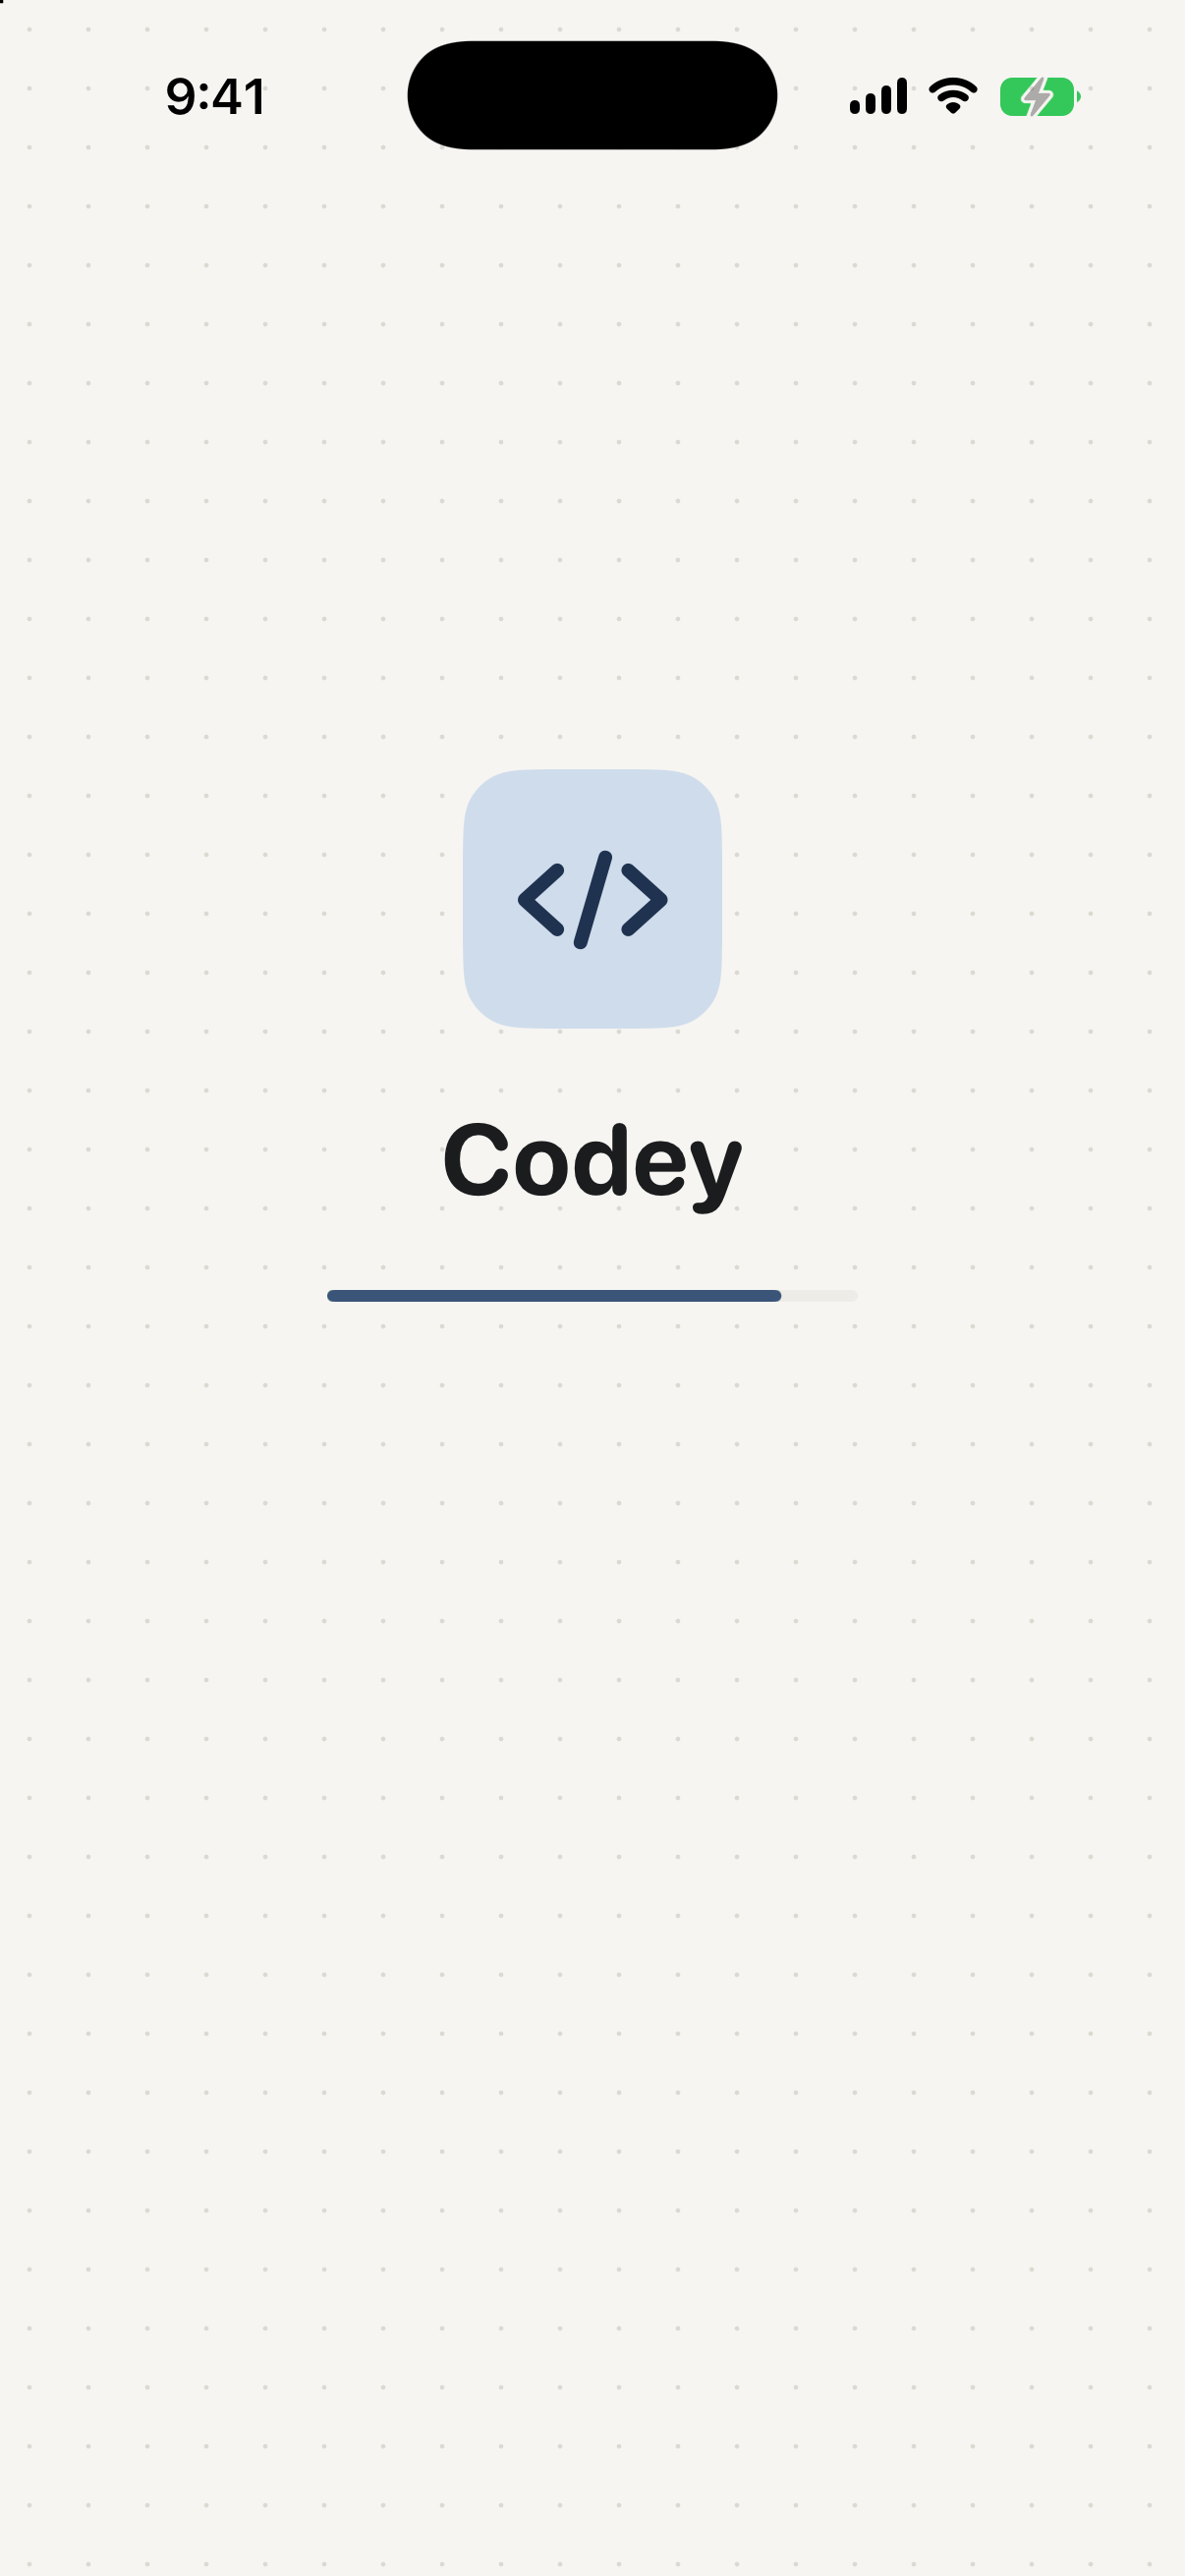
\includegraphics[width=0.235\textwidth]{launch.png}\hfill
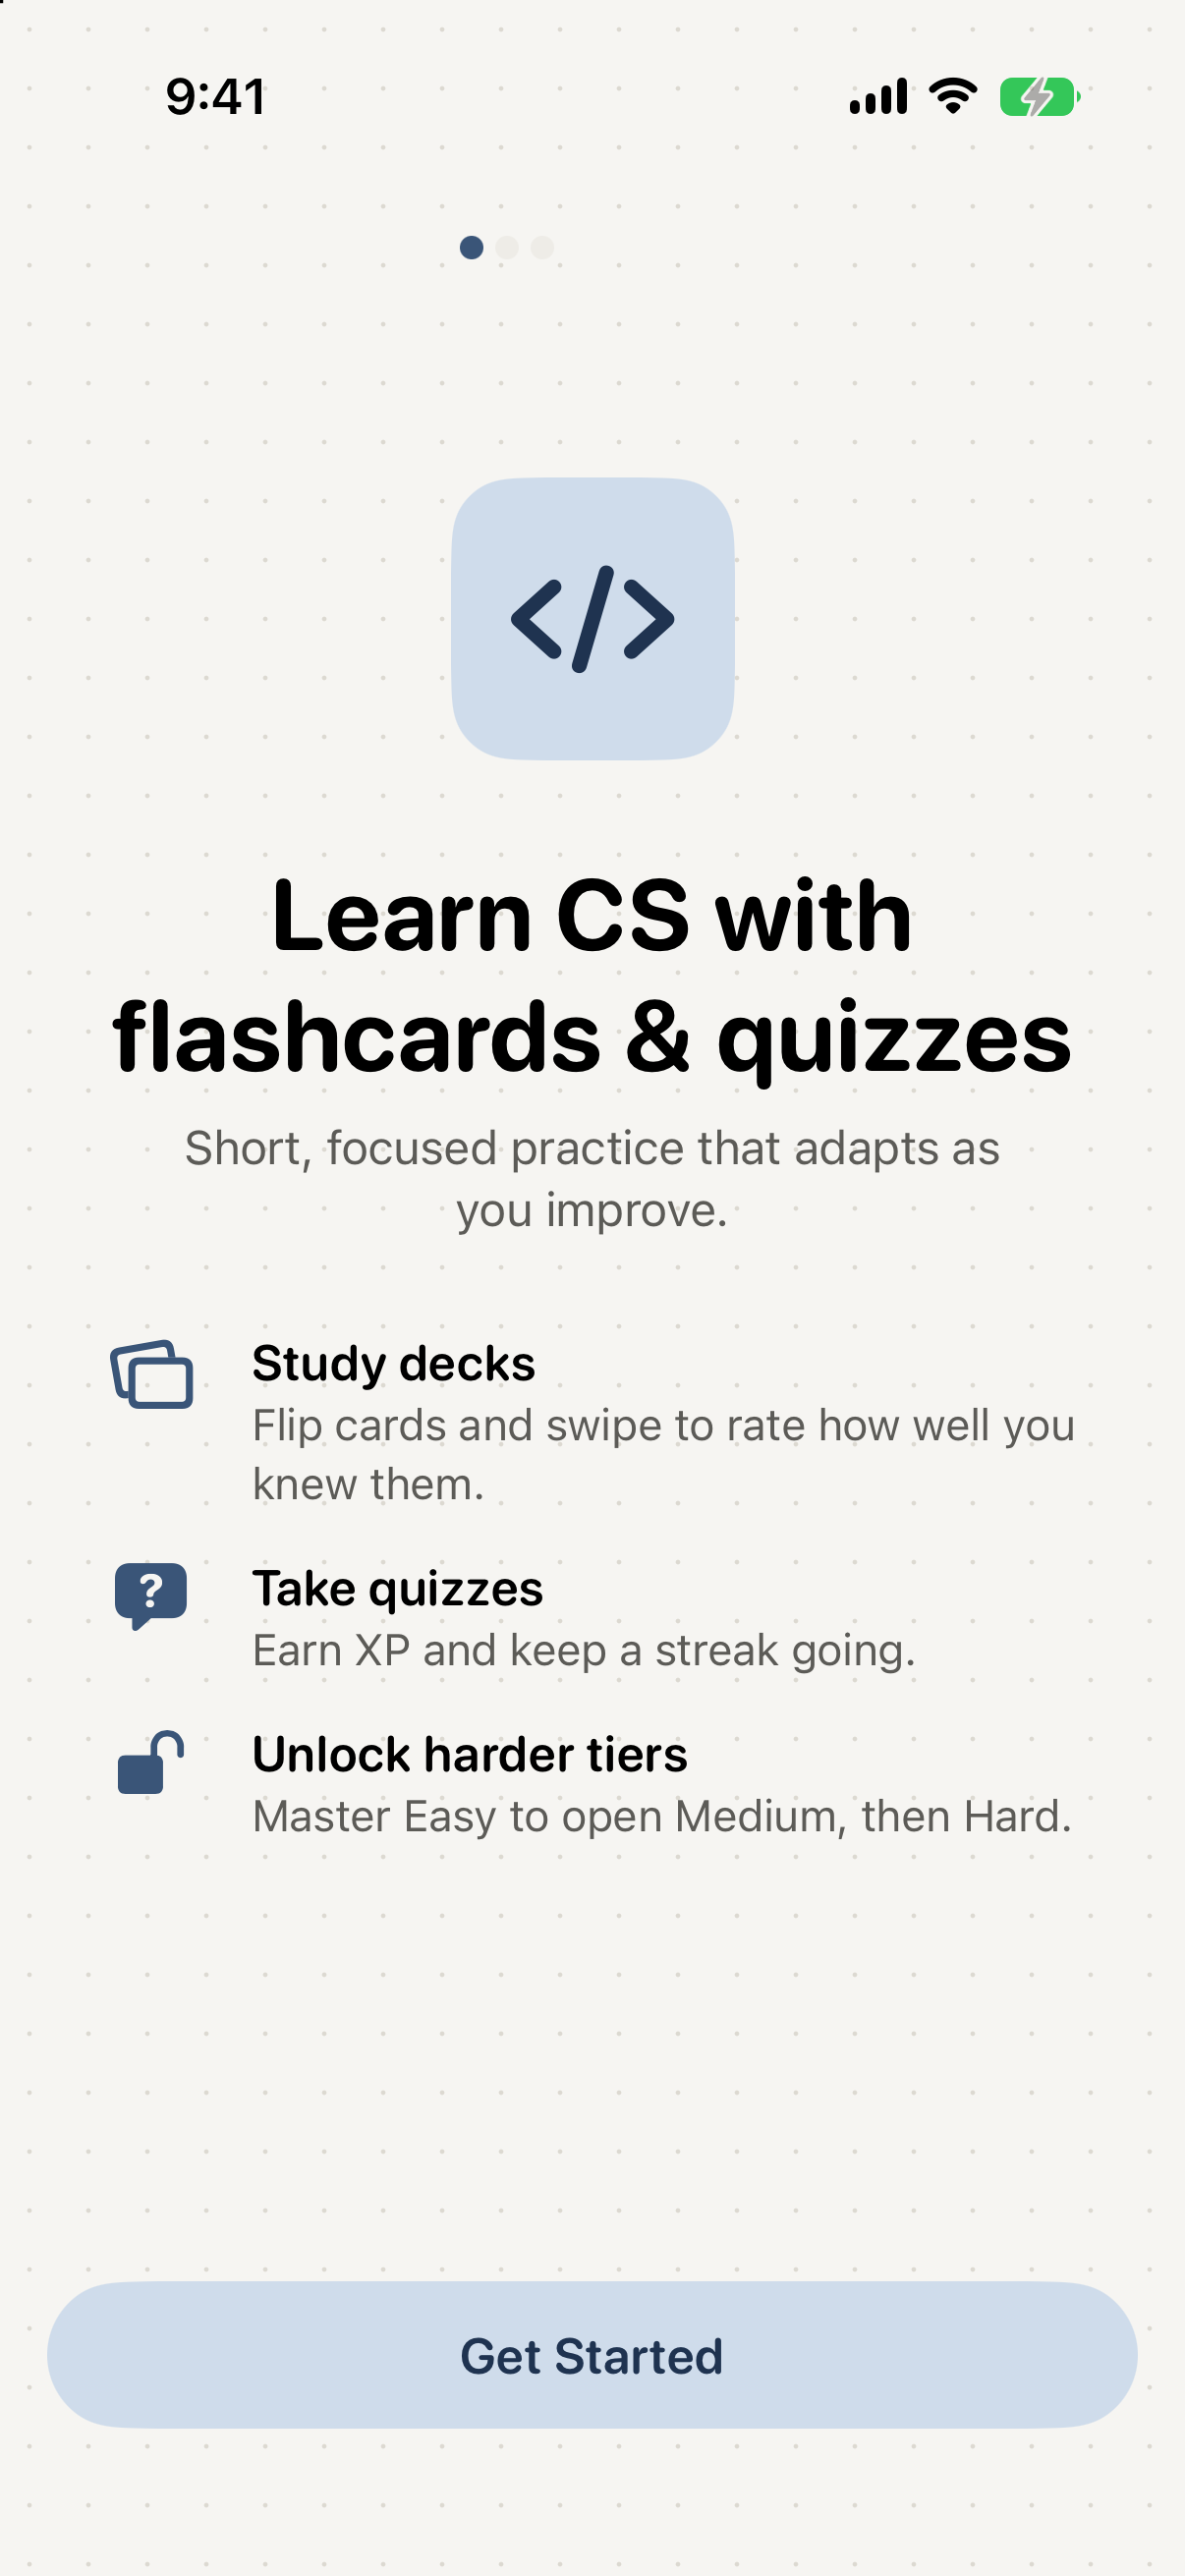
\includegraphics[width=0.235\textwidth]{onboarding.png}\hfill
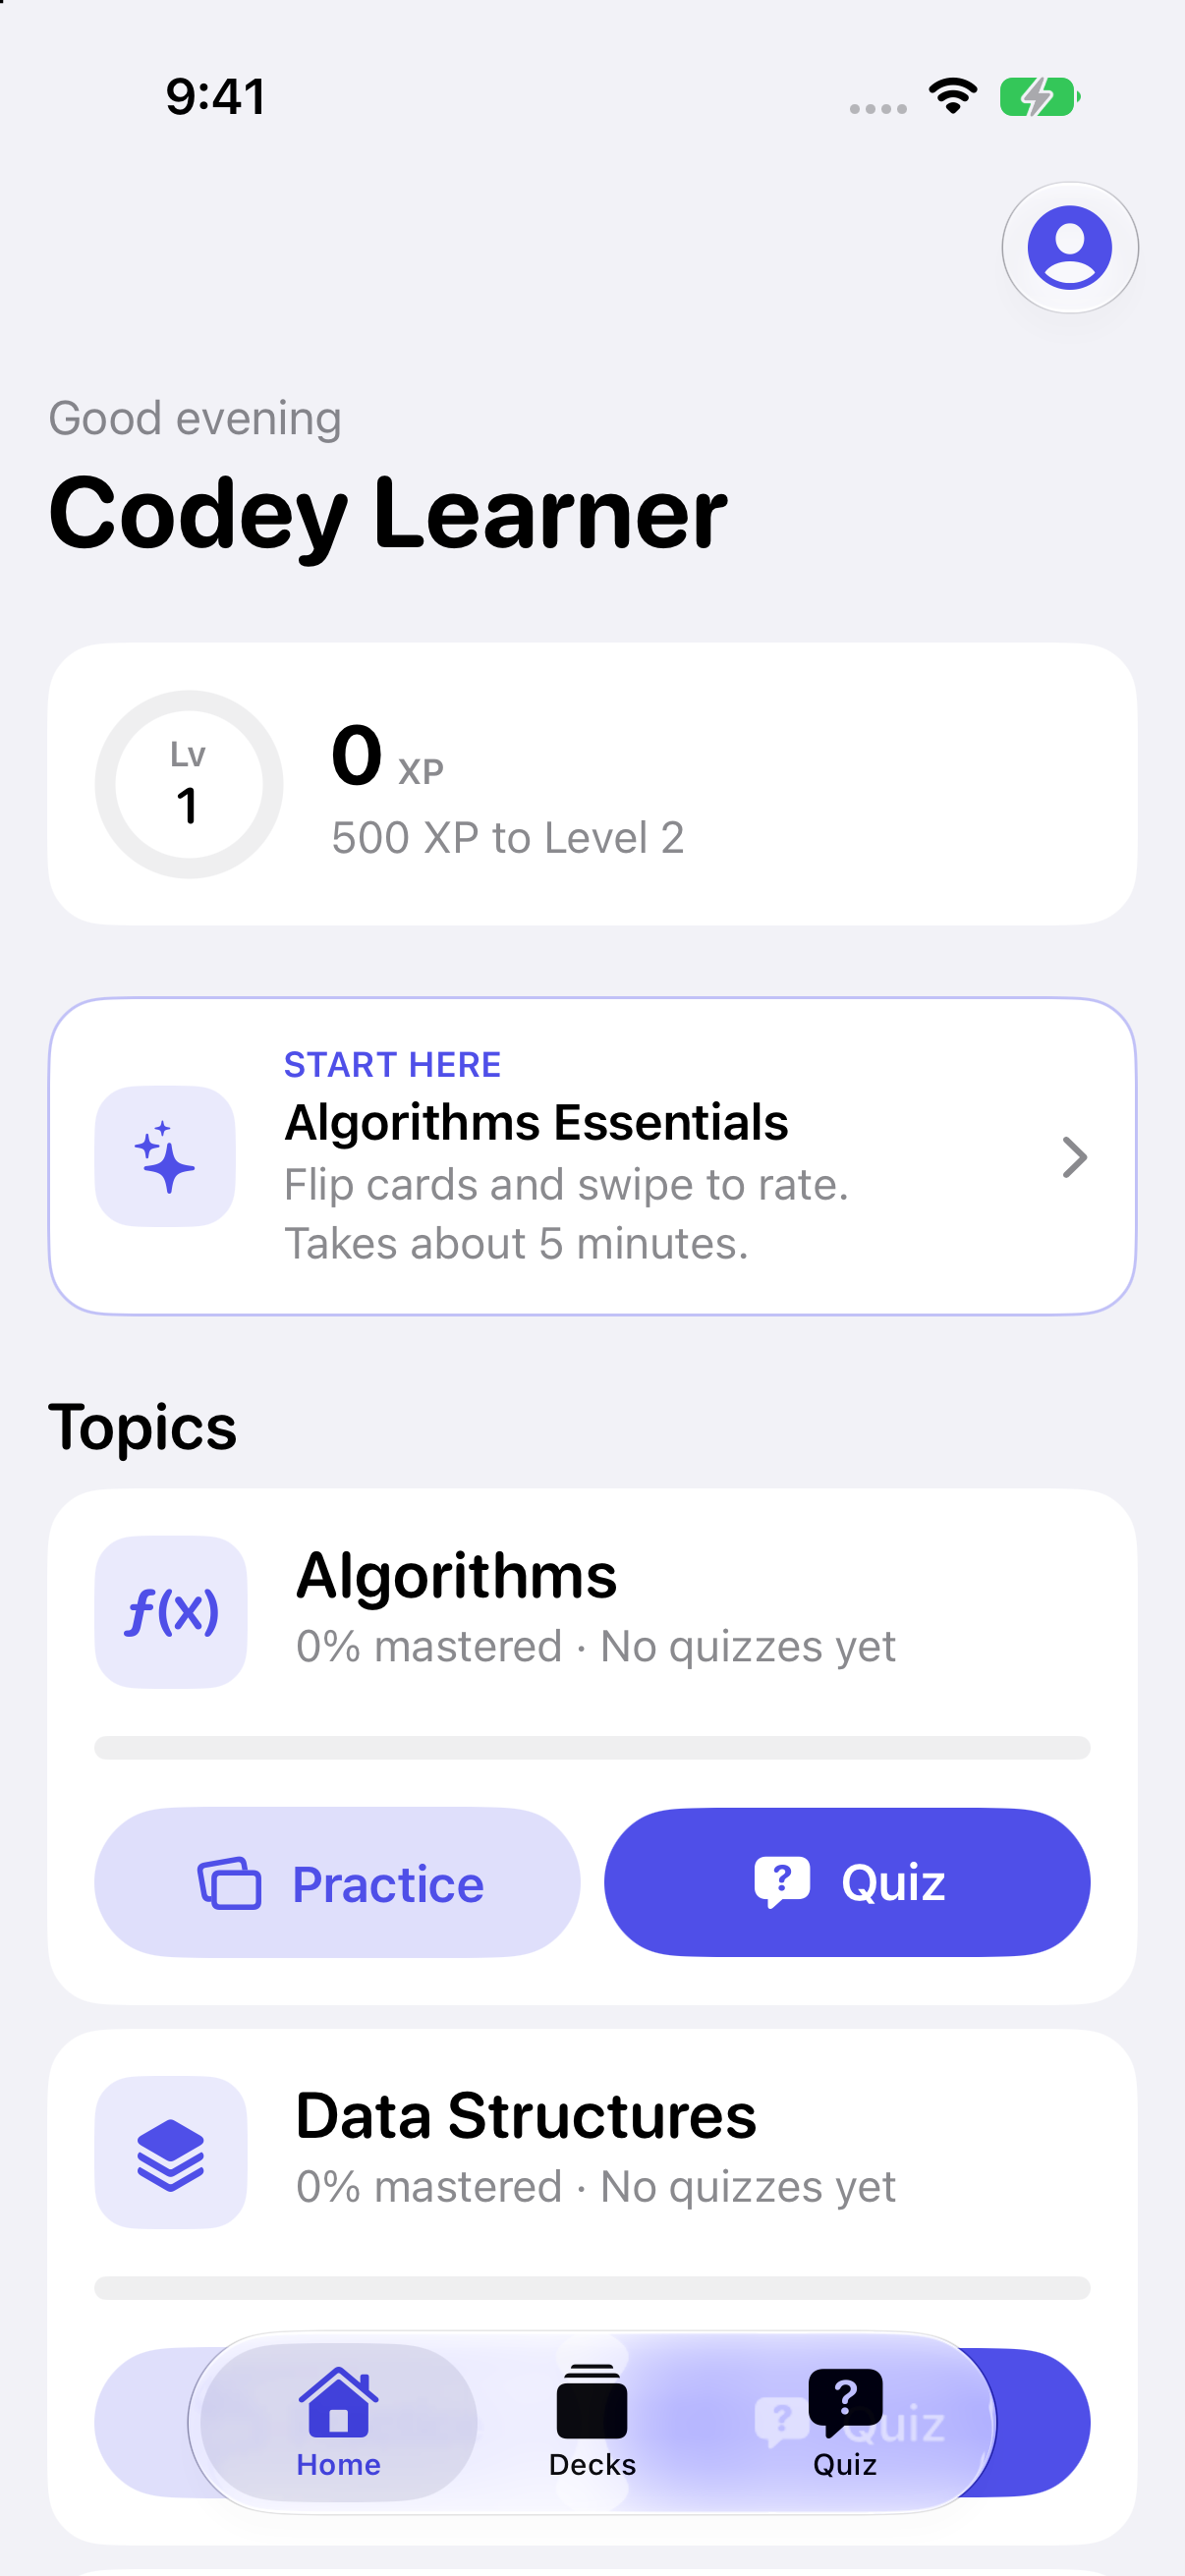
\includegraphics[width=0.235\textwidth]{home-light.png}\hfill
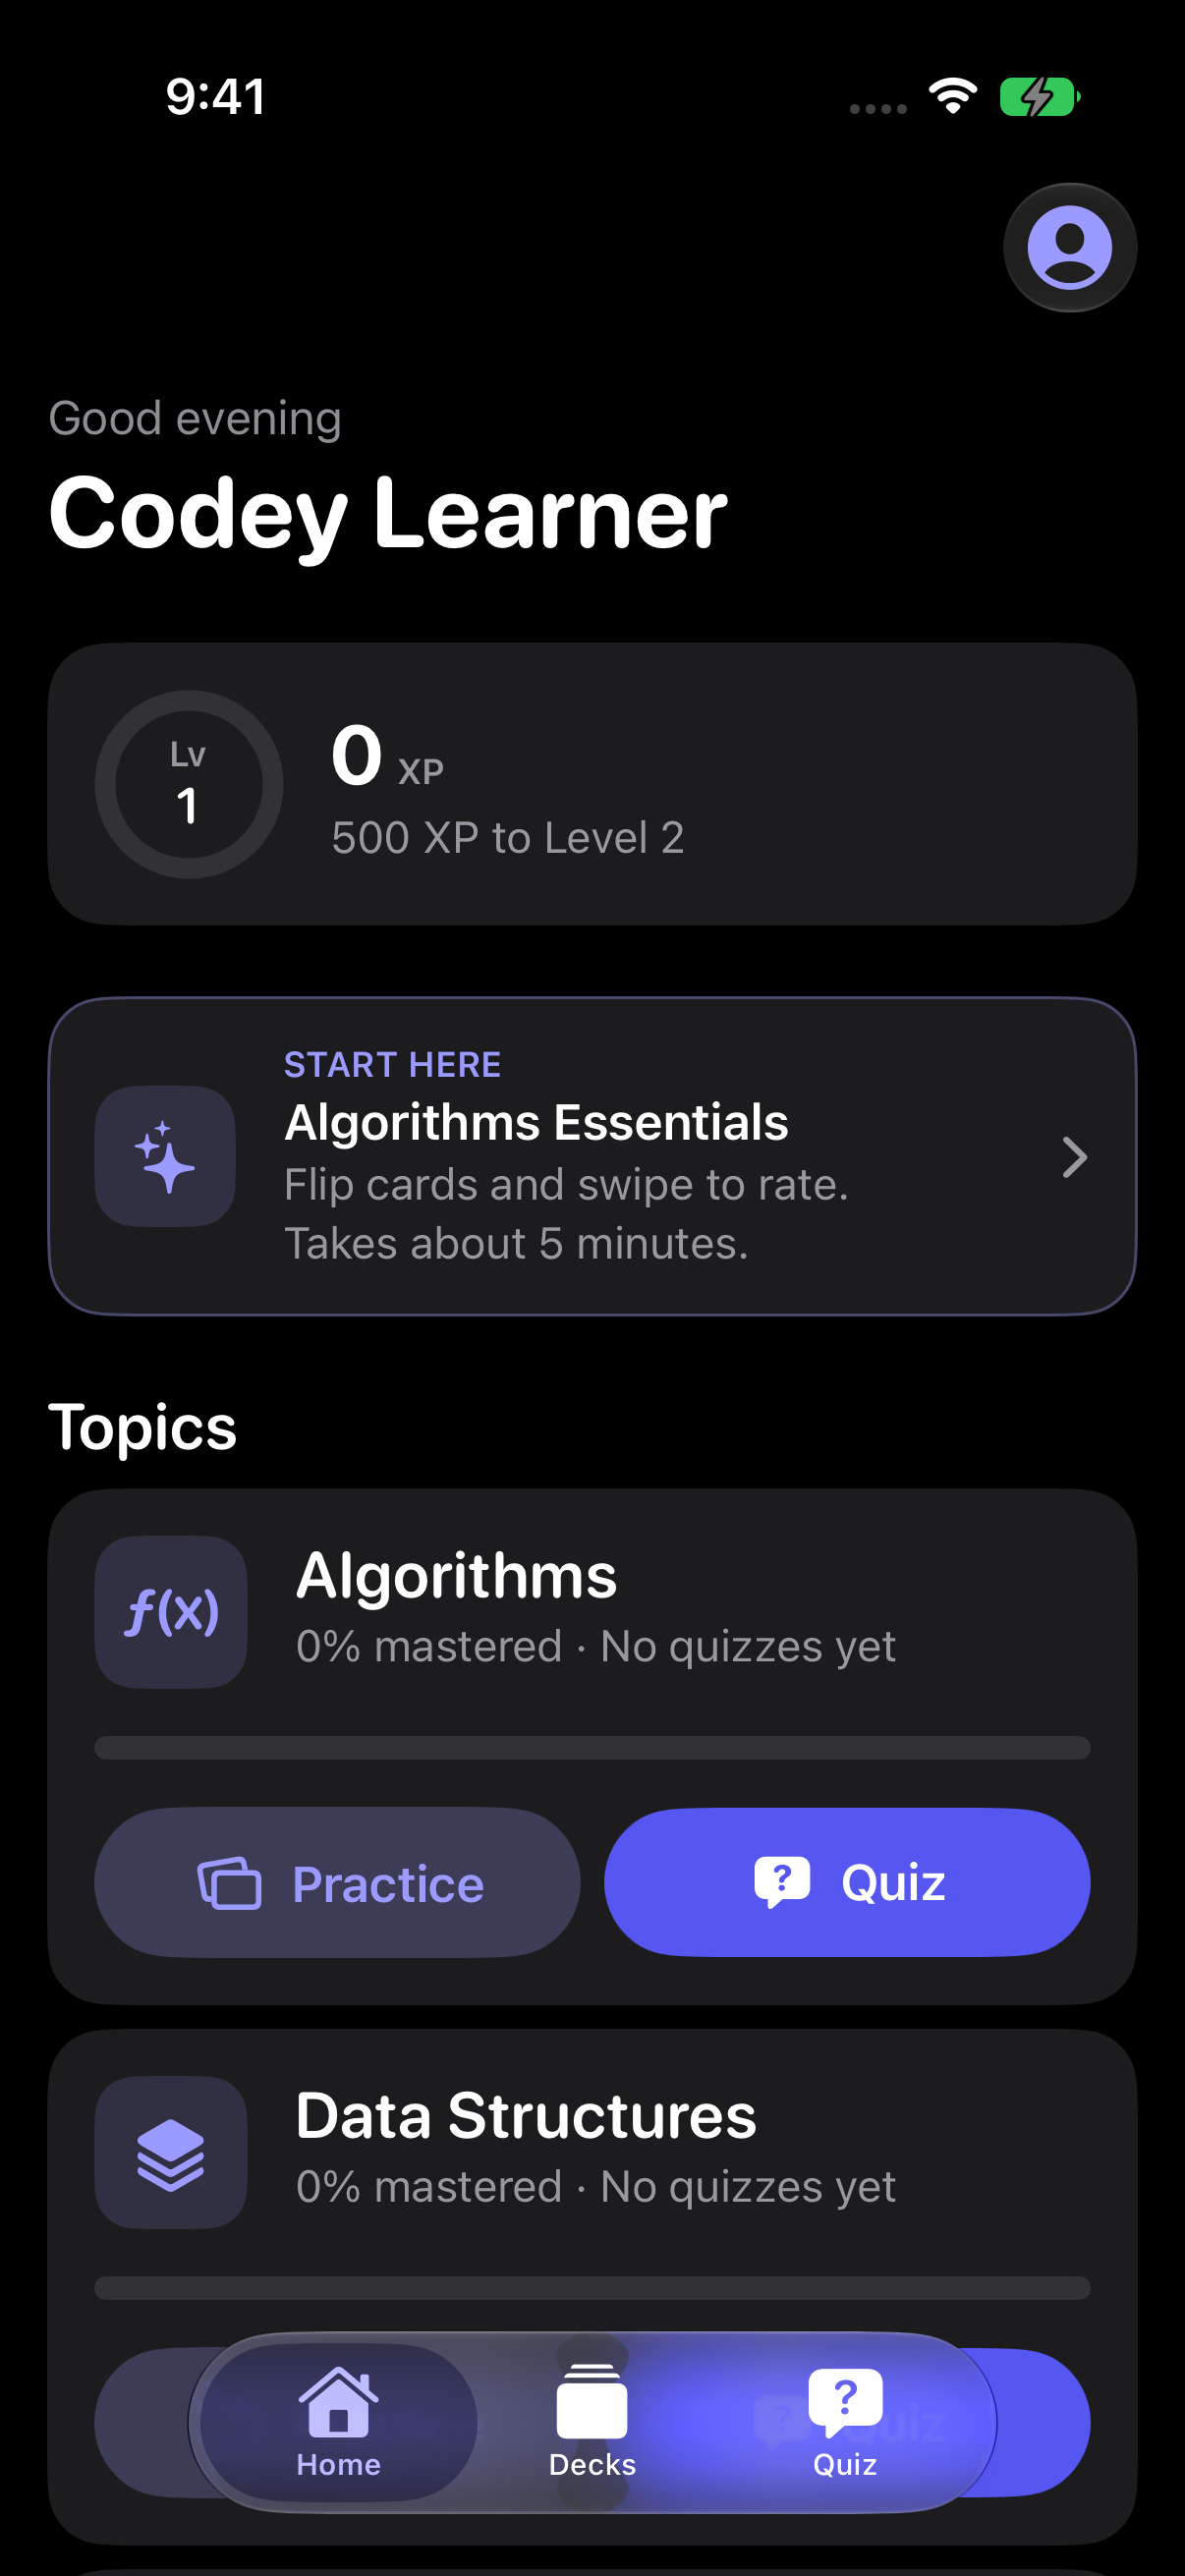
\includegraphics[width=0.235\textwidth]{home-dark.png}
\caption{Screens (iOS Simulator): launch, onboarding step 1, and Home in Light and Dark Mode}
\label{fig:screens}
\end{figure}

\subsection{Navigation Model}
The app is organized as a Home hub with a three-tab Liquid Glass tab bar (Home, Decks,
Quiz) that shrinks to a pill when the content scrolls (Figure~\ref{fig:nav}). Home shows
a greeting, the level card (level ring, XP, and XP to the next level), one ``Up next''
suggestion, and every topic with Practice and Quiz buttons. The suggestion is, in
priority order: resume a saved study session, start a starter deck (new learners), or
take a quiz on the weakest pinned topic. The avatar opens the profile sheet, an
inset-grouped list for the account, appearance (System, Light, Dark), pinned topics,
hidden starter decks, and the data reset actions. Studying and quizzing run as
full-screen covers (``focus mode''), so the tab bar never covers their controls. A
single router object owns every tab, sheet, and cover, so any screen can start a study
session or a quiz the same way.

\begin{figure}[!htbp]
\centering
\resizebox{\textwidth}{!}{%
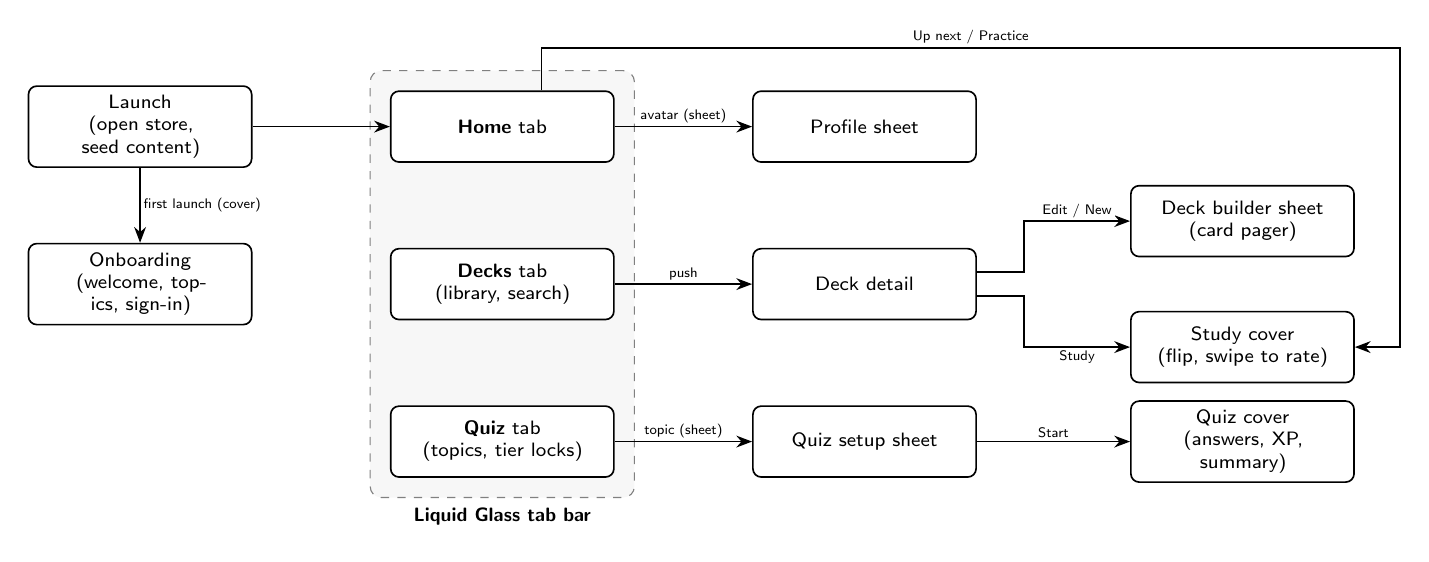
\begin{tikzpicture}[font=\sffamily\scriptsize,
    scr/.style={rectangle, rounded corners=3pt, draw, line width=0.6pt, fill=white,
                align=center, text width=2.6cm, minimum height=0.9cm},
    nav/.style={line width=0.6pt, -{Stealth[length=2mm]}},
    nl/.style={font=\sffamily\tiny, fill=white, inner sep=1pt}]
  \node[scr] (launch) at (-6.2,0)  {Launch\\(open store, seed content)};
  \node[scr] (onb)    at (-6.2,-2.0) {Onboarding\\(welcome, topics, sign-in)};
  \node[scr] (home)   at (-1.6,0)  {\textbf{Home} tab};
  \node[scr] (decks)  at (-1.6,-2.0) {\textbf{Decks} tab\\(library, search)};
  \node[scr] (quiz)   at (-1.6,-4.0) {\textbf{Quiz} tab\\(topics, tier locks)};
  \node[scr] (prof)   at (3.0,0)   {Profile sheet};
  \node[scr] (detail) at (3.0,-2.0) {Deck detail};
  \node[scr] (setup)  at (3.0,-4.0) {Quiz setup sheet};
  \node[scr] (build)  at (7.8,-1.2) {Deck builder sheet\\(card pager)};
  \node[scr] (study)  at (7.8,-2.8) {Study cover\\(flip, swipe to rate)};
  \node[scr] (qrun)   at (7.8,-4.0) {Quiz cover\\(answers, XP, summary)};
  \begin{scope}[on background layer]
    \node[draw=gray, dashed, rounded corners=4pt, fill=gray!6, inner sep=0.25cm,
          fit=(home)(decks)(quiz), label={[font=\sffamily\scriptsize\bfseries]below:Liquid Glass tab bar}] {};
  \end{scope}
  \draw[nav] (launch) -- (home);
  \draw[nav] (launch) -- node[nl, right] {first launch (cover)} (onb);
  \draw[nav] (home) -- node[nl, above] {avatar (sheet)} (prof);
  \draw[nav] (decks) -- node[nl, above] {push} (detail);
  \draw[nav] ([yshift=0.15cm]detail.east) -- ++(0.6,0) |- node[nl, above, pos=0.75] {Edit / New} (build.west);
  \draw[nav] ([yshift=-0.15cm]detail.east) -- ++(0.6,0) |- node[nl, below, pos=0.75] {Study} (study.west);
  \draw[nav] (quiz) -- node[nl, above] {topic (sheet)} (setup);
  \draw[nav] (setup) -- node[nl, above] {Start} (qrun);
  \draw[nav] ([xshift=0.5cm]home.north) |- (9.8,1.0) node[nl, pos=0.75, above] {Up next / Practice} |- (study.east);
\end{tikzpicture}}
\caption{Navigation model: tabs, sheets, and full-screen covers (a Home topic's Quiz button opens the same quiz setup sheet)}
\label{fig:nav}
\end{figure}

\subsection{Key Interactions}
\begin{itemize}
  \item \textbf{Onboarding} (first launch only) has three steps: a welcome screen,
        a topic picker that pins the chosen topics and their starter decks on Home,
        and an optional Google sign-in that can be skipped.
  \item \textbf{Deck builder.} A deck header (title with a character counter, topic
        picker) sits above a horizontal pager of card editors shaped like the study
        card, with a Front/Back toggle, a live Markdown preview, an optional code
        snippet edited in a syntax-highlighting code editor, and a final ``New card''
        page. A thumbnail strip below jumps to, reorders, duplicates, and deletes
        cards (with undo). Validation errors appear inline after the first failed save.
  \item \textbf{Study.} The card flips in 3D on tap (or Space); after the answer has
        been shown, a swipe rates it: left Again, down Hard, up Easy, right Good. The
        card is tinted with the rating's color while dragging, and a caption names the
        gestures. Keys 1--4 and VoiceOver actions on the card rate without gestures.
        Each rating has its own haptic.
  \item \textbf{Quiz.} A setup sheet shows the tier locks with their reasons (for
        example, ``Retire 3 more Medium questions'') and offers a mixed quiz or a single
        unlocked tier. During the quiz, a segmented progress bar, a streak chip, and a
        rolling XP total update after each answer; the summary shows the score ring and
        celebrates level-ups and tier unlocks.
\end{itemize}

\subsection{Design System}
Every screen is built from shared tokens and components (Table~\ref{tab:tokens}).
Screens never use raw colors, corner radii, or system fonts directly, and
\texttt{check-design-tokens.sh} enforces this. Shared components include buttons, cards,
chips, progress bars and rings, stat tiles, tier chips, answer rows, empty states, the
celebration overlay, and the form-feedback elements (inline field errors, character
counters, error outlines, and the error alert) used by every editor.

\begin{table}[H]
\centering
\caption{Design tokens and rules}
\label{tab:tokens}
\begin{tabularx}{\textwidth}{@{}L{2.4cm} Y@{}}
\toprule
\textbf{Area} & \textbf{Rule} \\
\midrule
Color & Electric-indigo brand (\texttt{\#4F4FE8} light, \texttt{\#9A9AFF} dark for text; a separate fill shade behind white labels), status colors, three tier colors, and eight syntax colors, each with a Dark Mode variant. Surfaces and text use iOS semantic colors. Every text/background pair passes 4.5:1, checked by a script and by a unit test (NFR-12). \\
Typography & Dynamic Type text styles throughout; SF Rounded for headings and numbers, with rolling digits for XP and counters; SF Mono for code. \\
Shape & Corner radii of 6, 10, 14, 20, and 28 points. Capsules only for single-line controls (chips, single-line buttons, progress bars); anything that can wrap uses a continuous rounded rectangle, and nested surfaces use concentric corners. \\
Materials & Liquid Glass on the control layer only (tab bar, floating buttons, toasts); content cards are solid raised surfaces. \\
Tiers & Easy, Medium, and Hard always pair a color with a symbol and a label, never color alone. \\
Motion & Standard snappy, bouncy, and smooth animations; under Reduce Motion every animation becomes a short crossfade. Particle bursts only for level-ups and tier unlocks. \\
Haptics & System \texttt{sensoryFeedback} for answers, ratings, saves, and celebrations. \\
Accessibility & VoiceOver labels and actions on every control, 44-point touch targets, Dynamic Type up to the accessibility sizes, and Light, Dark, or System appearance (NFR-11). \\
\bottomrule
\end{tabularx}
\end{table}

% =====================================================================
\section{UML Use Case Diagram}\label{sec:usecase}
% =====================================================================
Figure~\ref{fig:usecase} shows the use cases within the Codey system boundary. The
\emph{Student} is the primary actor. \emph{Local Data (SwiftData)} and \emph{Cloud
Sync (Supabase)} are secondary system actors responsible for persistence and
replication, and \emph{Google Account} is the external identity provider. The
diagram covers deck creation and synchronization together with quizzes, tiered
practice, starter decks, onboarding, and the profile.

\begin{figure}[!htbp]
\centering
\resizebox{\textwidth}{!}{%
\begin{tikzpicture}[font=\sffamily\scriptsize]
  % Use cases: student-facing (left column; the ends step left so actor lines clear)
  \node[usecase] (onboard)  at (-4.2,1.6)   {Onboard (Pick Topics)};
  \node[usecase] (create)   at (-3.6,0.0)   {Create / Edit Flashcard Deck};
  \node[usecase] (study)    at (-3.6,-1.6)  {Study Flashcard Deck};
  \node[usecase] (quiz)     at (-3.6,-3.2)  {Take Quiz};
  \node[usecase] (hide)     at (-3.6,-4.8)  {Hide / Restore Starter Deck};
  \node[usecase] (profile)  at (-3.6,-6.4)  {Manage Profile};
  \node[usecase] (report)   at (-4.2,-8.0)  {Report UI/UX Defect (planned)};
  % Middle column
  \node[usecase] (attach)   at (0.9,1.6)    {Attach Code Snippet};
  \node[usecase] (tier)     at (0.9,-2.4)   {Practice by Tier};
  \node[usecase] (signout)  at (0.6,-5.3)   {Sign Out};
  % System-facing (right column)
  \node[usecase] (validate) at (3.9,0.0)    {Validate Schema Constraints};
  \node[usecase] (cache)    at (3.9,-1.4)   {Cache Decks for Offline};
  \node[usecase] (queue)    at (3.9,-3.0)   {Queue Sync Transaction};
  \node[usecase] (repl)     at (3.9,-4.6)   {Replicate Decks to Remote};
  \node[usecase] (conflict) at (3.9,-6.2)   {Resolve Write Conflicts};
  \node[usecase] (auth)     at (3.9,-7.8)   {Authenticate User Session};
  % System boundary
  \begin{scope}[on background layer]
    \node[draw, line width=0.7pt, fill=magenta!5, inner sep=0.45cm,
          fit=(onboard)(attach)(create)(validate)(study)(quiz)(hide)(profile)(report)
              (tier)(signout)(auth)(cache)(queue)(repl)(conflict)] (sys) {};
  \end{scope}
  \node[anchor=north, font=\sffamily\scriptsize\bfseries] at (sys.north) {Codey Application Boundary};
  % Actors
  \pic at (-7.6,-3.6) {stickman};
  \node (student) at (-7.6,-3.6) [minimum width=0.6cm, minimum height=1.0cm] {};
  \node[below=0.05cm of student] {Student / User};
  \node[store] (local)  at (7.2,-0.8) {\st{system}\\Local Data\\(SwiftData)};
  \node[store] (cloud)  at (7.2,-4.6) {\st{system}\\Cloud Sync\\(Supabase)};
  \node[store] (google) at (7.2,-8.4) {\st{system}\\Google\\Account};
  % Associations
  \foreach \u in {onboard,create,study,quiz,hide,profile,report}
    \draw[line width=0.6pt] (student) -- (\u);
  \draw[line width=0.6pt] (validate) -- (local);
  \draw[line width=0.6pt] (cache)    -- (local);
  \draw[line width=0.6pt] (queue)    -- (local);
  \draw[line width=0.6pt] (queue)    -- (cloud);
  \draw[line width=0.6pt] (repl)     -- (cloud);
  \draw[line width=0.6pt] (conflict) -- (cloud);
  \draw[line width=0.6pt] (auth)     -- (cloud);
  \draw[line width=0.6pt] (auth)     -- (google);
  % Include / extend
  \tikzset{ucl/.style={font=\sffamily\scriptsize, inner sep=1pt}}
  \draw[dep] (attach)  -- node[ucl, above, sloped] {\st{extend}} (create);
  \draw[dep] (create)  -- node[lbl] {\st{include}} (validate);
  \draw[dep] (tier)    -- node[ucl, below, sloped] {\st{extend}} (quiz);
  \draw[dep] (tier)    -- node[ucl, above, sloped] {\st{extend}} (study);
  \draw[dep] (signout) -- node[ucl, above, sloped] {\st{extend}} (profile);
  \draw[dep] (profile) -- node[ucl, below, sloped, pos=0.55] {\st{include}} (auth);
  \draw[dep] (conflict) -- node[ucl, right] {\st{extend}} (repl);
\end{tikzpicture}}
\caption{UML use case diagram: Codey decks, study, quizzes, profile, and synchronization}
\label{fig:usecase}
\end{figure}

\textbf{Actors.} The \emph{Student} completes onboarding, creates, edits, and studies
decks, takes quizzes, hides or restores starter decks, manages the profile, and (in a
later sprint) submits defect reports. \emph{Local Data} validates and persists cards,
caches decks for offline use, and records unsynchronized changes. \emph{Cloud Sync}
authenticates sessions, replicates decks across devices, and resolves write conflicts.
\emph{Google Account} verifies the student's identity for sign-in.

\textbf{Relationships.} \emph{Create / Edit Flashcard Deck} includes \emph{Validate
Schema Constraints}, because no card is saved until it conforms to the JSON card schema
(FR-09). \emph{Attach Code Snippet} extends it with an optional syntax-highlighted
example (FR-07, FR-08). \emph{Practice by Tier} extends both \emph{Take Quiz} and
\emph{Study Flashcard Deck} when the student restricts a session to one unlocked tier
(FR-29). \emph{Manage Profile} includes \emph{Authenticate User Session} for sign-in,
and \emph{Sign Out} extends it (FR-03). \emph{Resolve Write Conflicts} extends
\emph{Replicate Decks to Remote} and runs only when, at push time, the remote copy has
changed since this device's last synchronization (FR-47). Sign-in is optional:
every use case except \emph{Replicate Decks to Remote} works for a guest.

Table~\ref{tab:uc01} specifies UC-01 in full. The traceability matrix
(Section~\ref{sec:trace}) uses the following use case identifiers: UC-01 Create / Edit
Flashcard Deck, UC-02 Attach Code Snippet, UC-03 Validate Schema Constraints, UC-04
Study Flashcard Deck, UC-05 Report UI/UX Defect, UC-06 Replicate Decks to Remote, UC-07
Queue Sync Transaction, UC-08 Authenticate User Session, UC-09 Cache Decks for Offline,
UC-10 Resolve Write Conflicts, UC-11 Take Quiz, UC-12 Practice by Tier, UC-13 Hide /
Restore Starter Deck, UC-14 Onboard, UC-15 Manage Profile, and UC-16 Sign Out.

\begin{table}[H]
\centering
\caption{Use case specification: UC-01 Create / Edit Flashcard Deck}
\label{tab:uc01}
\begin{tabularx}{\textwidth}{@{}L{3.0cm} Y@{}}
\toprule
\textbf{Field} & \textbf{Description} \\
\midrule
Primary actor & Student \\
Secondary actors & Local Data (SwiftData); Cloud Sync (Supabase) \\
Preconditions & The app is running and the student is on the deck library screen. Sign-in is not required. \\
Main flow & 1. The student selects \emph{New Deck}; the builder opens an in-memory draft (no deck exists in the store yet). 2. The student enters a title, a topic, and one or more prompt/answer cards. 3. The student selects \emph{Save}. 4. The system validates the deck and every card (UC-03). 5. The system creates the deck and its cards through \texttt{FlashcardFactory} and saves them locally; the deck passes through \emph{Drafting} into \emph{LocallyPersisted}. 6. The system queues the deck and its cards for synchronization (UC-07), schedules a sync two seconds later, and returns to the library. \\
Alternate flows & 2a. The student attaches a code snippet (UC-02). 4a. Validation fails: the system shows inline errors, moves to the first invalid card, and remains on the form; after the first failed save, errors update as the student types. 6a. The device is offline or the student is a guest: the changes stay queued until connectivity is restored or the student signs in. \\
Postconditions & The deck exists in SwiftData and appears in the library with its sync status. \\
Requirements & FR-05, FR-06, FR-07, FR-09, FR-10, FR-11, FR-44, FR-45, FR-48 \\
\bottomrule
\end{tabularx}
\end{table}

% =====================================================================
\section{Requirements Traceability Table}\label{sec:trace}
% =====================================================================

Table~\ref{tab:rtm} traces each functional requirement to the use case that motivates
it, the design elements that realize it, and the test case that verifies it. Test case
identifiers correspond to requirement numbers (TC-05 verifies FR-05), and
Table~\ref{tab:tcmap} maps each test case to the automated test suites that implement
it. Requirements that share a use case, design element, and status are grouped in a
single row but keep individual test case identifiers. A dash indicates that no use case
covers the requirement. Design elements are the type and member names used in the code.

\begin{xltabular}{\textwidth}{@{}l L{1.6cm} Y l l@{}}
\caption{Requirements traceability matrix}\label{tab:rtm}\\
\toprule
\textbf{Req.} & \textbf{Use Case} & \textbf{Design Element(s)} & \textbf{Test} & \textbf{Status} \\
\midrule
\endfirsthead
\multicolumn{5}{@{}l}{\small\itshape Table \thetable\ continued} \\
\toprule
\textbf{Req.} & \textbf{Use Case} & \textbf{Design Element(s)} & \textbf{Test} & \textbf{Status} \\
\midrule
\endhead
\bottomrule
\endfoot
FR-01 & UC-08 & \texttt{BackendFacade.signInWithGoogle()}, \texttt{SupabaseAuthProvider} (\texttt{AuthProviding}) & TC-01 & Implemented \\
FR-02 & UC-08 & \texttt{KeychainSessionStorage} (Supabase session storage); iOS Keychain artifact (Fig.~\ref{fig:deploy}) & TC-02 & Implemented \\
FR-03 & UC-16 & \texttt{BackendFacade.signOut(\allowbreak removingLocalDecks:)}, \texttt{SupabaseAuthProvider.signOut()} & TC-03 & Implemented \\
FR-04 & UC-15 & \texttt{profiles} table (\texttt{display\_name}, \texttt{avatar\_id}) synced by \texttt{SyncEngine}; no editor or avatar picker yet & TC-04 & Planned \\
FR-05 & UC-01 & \texttt{DeckBuilderView}, \texttt{DeckViewModel.createDeck()}, \texttt{ModelValidator.validateDeck()}, \texttt{FlashcardDeck} & TC-05 & Implemented \\
FR-06 & UC-01 & \texttt{FlashcardFactory.createCard()}, \texttt{SwiftDataService.apply()} & TC-06 & Implemented \\
FR-07 & UC-02 & \texttt{CodeSnippet}, \texttt{CodeEditorView}, \texttt{FlashcardFactory} & TC-07 & Implemented \\
FR-08 & UC-02 & \texttt{CardMarkdownView} (Textual, Prism.js), \texttt{CodeEditorView} (Runestone, Tree-sitter), \texttt{SyntaxRole} & TC-08 & Implemented \\
FR-09 & UC-03 & \texttt{ModelValidator.validateCard()}, \texttt{FlashcardPayload}, \texttt{flashcard.schema.json} & TC-09 & Implemented \\
FR-10 & UC-03 & \texttt{DeckViewModel.fieldErrors}, \texttt{FieldErrorLabel}; \emph{Drafting} self-transition (Fig.~\ref{fig:state}) & TC-10 & Implemented \\
FR-11 & UC-01 & \texttt{DeckViewModel.updateDeck()}, \texttt{FlashcardFactory.updateCard()}; \emph{Drafting} state & TC-11 & Implemented \\
FR-12 & UC-01 & \texttt{BackendFacade.deleteDeck()}, \texttt{DeckSyncState.onDelete()} (tombstone), delete operation in \texttt{SyncQueue}; final state ``Deck removed'' & TC-12 & Implemented \\
FR-13 & UC-01 & \texttt{DeckViewModel.deleteCard()} (in the builder), \texttt{BackendFacade.deleteCard()} & TC-13 & Implemented \\
FR-14 & -- & \texttt{StarterDeckLoader}, \texttt{FlashcardFactory.createCard(from:)}, \texttt{starter-decks.json} & TC-14 & Implemented \\
FR-15 & UC-13 & \texttt{BackendFacade.setHidden(\_:deck:)}, \texttt{DeckLibraryView}, profile sheet & TC-15 & Implemented \\
FR-16 -- FR-18 & UC-04 & \texttt{StudySessionViewModel}, \texttt{StudyQueue}, \texttt{Flashcard.updateMastery(rating:)}, \texttt{CardRating} & TC-16 -- TC-18 & Implemented \\
FR-19 -- FR-21 & UC-11 & \texttt{QuizViewModel}, \texttt{QuestionPool.build()}, \texttt{QuestionBankLoader} & TC-19 -- TC-21 & Implemented \\
FR-22 -- FR-29 & UC-11, UC-12 & \texttt{QuizProgressStore}, \texttt{QuestionProgress}, \texttt{TopicProgress}, \texttt{TierGate}, \texttt{QuestionPool}, \texttt{StudyPool}, \texttt{GatingConfig} & TC-22 -- TC-29 & Implemented \\
FR-30 -- FR-31 & UC-11 & \texttt{XPPolicy}, \texttt{LevelCalculator}, \texttt{QuizViewModel.select()} & TC-30 -- TC-31 & Implemented \\
FR-32 -- FR-35 & -- & \texttt{DailyActivity} records cards rated and quiz answers per day; streak, daily goal, and badge rules not built & TC-32 -- TC-35 & Planned \\
FR-36 & UC-11 & \texttt{QuizAnswerRecord}, \texttt{QuizProgressStore.accuracy()} & TC-36 & Implemented \\
FR-37 & -- & \texttt{HomeView} (level card, topic cards with per-topic accuracy) & TC-37 & Implemented \\
FR-38 & -- & \texttt{HomeLogic.weakestTopicID()} suggests one quiz; the weekly three-topic plan is not built & TC-38 & In progress \\
FR-39 -- FR-41 & -- & Exercise editor and validator that compares each blank with its accepted solutions; no code is executed on the device & TC-39 -- TC-41 & Planned \\
FR-42 -- FR-43 & -- & Leaderboard and weekly-challenge tables in Supabase, protected by RLS, read through \texttt{BackendFacade} & TC-42 -- TC-43 & Planned \\
FR-44 & UC-09 & \texttt{BackendFacade.saveDeck()}, \texttt{SwiftDataService.apply()} & TC-44 & Implemented \\
FR-45 & UC-07 & \texttt{SyncQueue} (coalescing), \texttt{SyncOperation} & TC-45 & Implemented \\
FR-46 & UC-06 & \texttt{SyncEngine} (push, pull, backoff), \texttt{RemoteChangeApplier}, \texttt{NetworkMonitor} & TC-46 & Implemented \\
FR-47 & UC-10 & \texttt{ConflictResolver.merge()}, \texttt{ConflictState.onResolve()} & TC-47 & Implemented \\
FR-48 & UC-06 & \texttt{DeckStatusChip}, \texttt{DeckSyncStateKind.displayName}; state machine (Fig.~\ref{fig:state}) & TC-48 & Implemented \\
FR-49 & UC-05 & -- & TC-49 & Planned \\
\end{xltabular}

Non-functional requirements describe system qualities rather than user goals.
Table~\ref{tab:rtm-nfr} therefore traces each one to the architectural element that
satisfies it (component, deployment node, or class) and to its verification test.

\begin{xltabular}{\textwidth}{@{}l L{3.2cm} Y l l@{}}
\caption{Non-functional requirements traceability matrix}\label{tab:rtm-nfr}\\
\toprule
\textbf{Req.} & \textbf{Quality} & \textbf{Satisfied By (Design Element)} & \textbf{Test} & \textbf{Status} \\
\midrule
\endfirsthead
\multicolumn{5}{@{}l}{\small\itshape Table \thetable\ continued} \\
\toprule
\textbf{Req.} & \textbf{Quality} & \textbf{Satisfied By (Design Element)} & \textbf{Test} & \textbf{Status} \\
\midrule
\endhead
\bottomrule
\endfoot
NFR-01 & Dashboard load $\le$ 3 s & Local-first reads from the SwiftData store (Local Store component, Fig.~\ref{fig:component}); no network wait on launch & TC-N01 & Planned \\
NFR-02 & 100-card sync $\le$ 5 s & \texttt{SyncEngine} batched push (one request per table, up to 500 operations); PostgREST (Fig.~\ref{fig:deploy}) & TC-N02 & In progress \\
NFR-03 & Latest iOS, target iOS 26 & Client node (Fig.~\ref{fig:deploy}); Xcode deployment target & TC-N03 & Implemented \\
NFR-04 & Local encryption at rest & SwiftData store with \emph{complete unless open} protection; Keychain item \emph{this device only} (Fig.~\ref{fig:deploy}) & TC-N04 & Implemented \\
NFR-05 & Cloud encryption at rest & Data tier node: managed PostgreSQL instance (Fig.~\ref{fig:deploy}) & TC-N05 & Implemented \\
NFR-06 & TLS 1.3 in transit & \texttt{SupabaseServices.tlsConfiguration} (minimum TLS 1.3); HTTPS path on port 443 (Fig.~\ref{fig:deploy}) & TC-N06 & Implemented \\
NFR-07 & Row-level data ownership & RLS policies on all four tables, enforced by PostgREST (Fig.~\ref{fig:deploy}) & TC-N07 & Implemented \\
NFR-08 & Offline quizzes and flashcards & Local Store component; local-only \texttt{BackendFacade} when signed out or unconfigured; save-local-first sequence (Fig.~\ref{fig:sequence}) & TC-N08 & Implemented \\
NFR-09 & Reliable sync within 30 s & \texttt{SyncQueue}, \texttt{SyncEngine} reconnect trigger, \texttt{NetworkMonitor} (\texttt{Reachability}); State pattern (Fig.~\ref{fig:statepattern}) & TC-N09 & Implemented \\
NFR-10 & Consistent layout across screen sizes & Presentation component (SwiftUI adaptive layouts, \texttt{ViewThatFits}) & TC-N10 & In progress \\
NFR-11 & Light and Dark Mode & \texttt{AppAppearance} (System, Light, Dark); asset colors with dark variants & TC-N11 & In progress \\
NFR-12 & 4.5:1 text contrast & Design-system color tokens (Section~\ref{sec:ui}) & TC-N12 & In progress \\
NFR-13 & Uses a database & Local Store component and PostgreSQL (Figs.~\ref{fig:component} and~\ref{fig:deploy}) & TC-N13 & Implemented \\
NFR-14 & Swift/SwiftUI with Xcode & \texttt{Codey.app} artifact on the client node (Fig.~\ref{fig:deploy}) & TC-N14 & Implemented \\
NFR-15 & Team-written source code & All components; GitHub pull request workflow (Section~\ref{sec:process}) & TC-N15 & Implemented \\
NFR-16 & 70\% unit-test coverage & Model, ViewModel, and Service layers (89.3\%) & TC-N16 & Implemented \\
NFR-17--19 & Metrics every sprint & Metrics plan (Table~\ref{tab:metrics}) & TC-N17--19 & In progress \\
NFR-20 & No service costs & Free plans and open-source libraries (Table~\ref{tab:services}) & TC-N20 & Implemented \\
\end{xltabular}

\begin{xltabular}{\textwidth}{@{}L{2.4cm} Y@{}}
\caption{Test cases mapped to automated test suites}\label{tab:tcmap}\\
\toprule
\textbf{Test case} & \textbf{Suites (Swift Testing; the two XCTest UI tests are marked UI)} \\
\midrule
\endfirsthead
\multicolumn{2}{@{}l}{\small\itshape Table \thetable\ continued} \\
\toprule
\textbf{Test case} & \textbf{Suites} \\
\midrule
\endhead
\bottomrule
\endfoot
TC-01, TC-03 & \texttt{SyncEngineTests} (sign-in claims guest decks, cancelled sign-in, sign-out keeping or removing decks) \\
TC-02 & \texttt{KeychainSessionStorageTests} \\
TC-05 -- TC-07, TC-11, TC-13 & \texttt{DeckViewModelTests}, \texttt{FlashcardFactoryTests}, \texttt{DeckBuilderUITests} (UI) \\
TC-08 & \texttt{CardMarkdownCompositionTests}, \texttt{SyntaxRoleTests}, \texttt{MarkdownFormattingTests} \\
TC-09, TC-10 & \texttt{ModelValidatorTests}, \texttt{FlashcardSchemaFileTests}, \texttt{SupabaseSchemaTests}, \texttt{DeckViewModelTests} \\
TC-12 & \texttt{DeckSyncStateTests}, \texttt{SyncEngineTests} (delete tests) \\
TC-14 & \texttt{StarterDeckLoaderTests}, \texttt{DataSeederTests} \\
TC-15 & \texttt{DeckViewModelTests} (starter decks can be hidden, not edited or deleted) \\
TC-16 -- TC-18 & \texttt{StudySessionViewModelTests}, \texttt{StudyQueueTests}, \texttt{SwipeRatingTests}, \texttt{CardRatingTests}, \texttt{FlashcardMasteryTests}, \texttt{StudySessionUITests} (UI) \\
TC-19 -- TC-21 & \texttt{QuizViewModelTests}, \texttt{QuestionPoolTests}, \texttt{QuestionBankLoaderTests} \\
TC-22 -- TC-29 & \texttt{QuestionProgressTests}, \texttt{TierGateTests}, \texttt{StudyPoolTests}, \texttt{QuestionPoolTests}, \texttt{QuizViewModelTests} \\
TC-30, TC-31 & \texttt{XPPolicyTests}, \texttt{LevelCalculatorTests}, \texttt{QuizViewModelTests} \\
TC-36 & \texttt{QuizViewModelTests} (accuracy over the last 50 answers) \\
TC-37, TC-38 & \texttt{HomeLogicTests}, \texttt{RouterTests} \\
TC-44 & \texttt{DeckViewModelTests}, \texttt{SyncEngineTests} (offline save never touches the network) \\
TC-45 & \texttt{SyncQueueTests} \\
TC-46 & \texttt{SyncEngineTests} (push, pull, backoff, reconnect), \texttt{SupabaseDataClientTests} \\
TC-47 & \texttt{ConflictResolverTests}, \texttt{SyncEngineTests} (concurrent edits, two devices converge) \\
TC-48 & \texttt{DeckSyncStateTests} \\
TC-N02 & \texttt{SyncEngineTests} (one request per table), \texttt{SupabaseIntegrationTests} (opt-in, timed) \\
TC-N04 & \texttt{StoreFileProtectionTests}, \texttt{KeychainSessionStorageTests} \\
TC-N06 & \texttt{TransportSecurityTests}, \texttt{AppConfigTests} \\
TC-N07 & \texttt{SupabaseSchemaTests} (every table has RLS), \texttt{supabase/tests/rls.sql}, \texttt{SupabaseIntegrationTests} (opt-in) \\
TC-N08, TC-N09 & \texttt{SyncEngineTests} (offline save, reconnect), \texttt{SupabaseIntegrationTests} (opt-in) \\
TC-N11, TC-N12 & \texttt{ColorTokenTests}, \texttt{ContrastTests}, \texttt{AppAppearanceTests} \\
TC-N13 & \texttt{MigrationTests}, \texttt{DataSeederTests}, \texttt{LocalDataResetTests} \\
TC-N16 & Coverage report (\texttt{xccov}) on every test run \\
\end{xltabular}

Each pull request references the requirement identifiers it affects, and the Project
Manager updates the Status column when the associated test passes. Every design element
in these models traces to at least one requirement.

% =====================================================================
\section{UML Sequence Diagram}
% =====================================================================

\begin{figure}[!htbp]
\centering
\resizebox{\textwidth}{!}{%
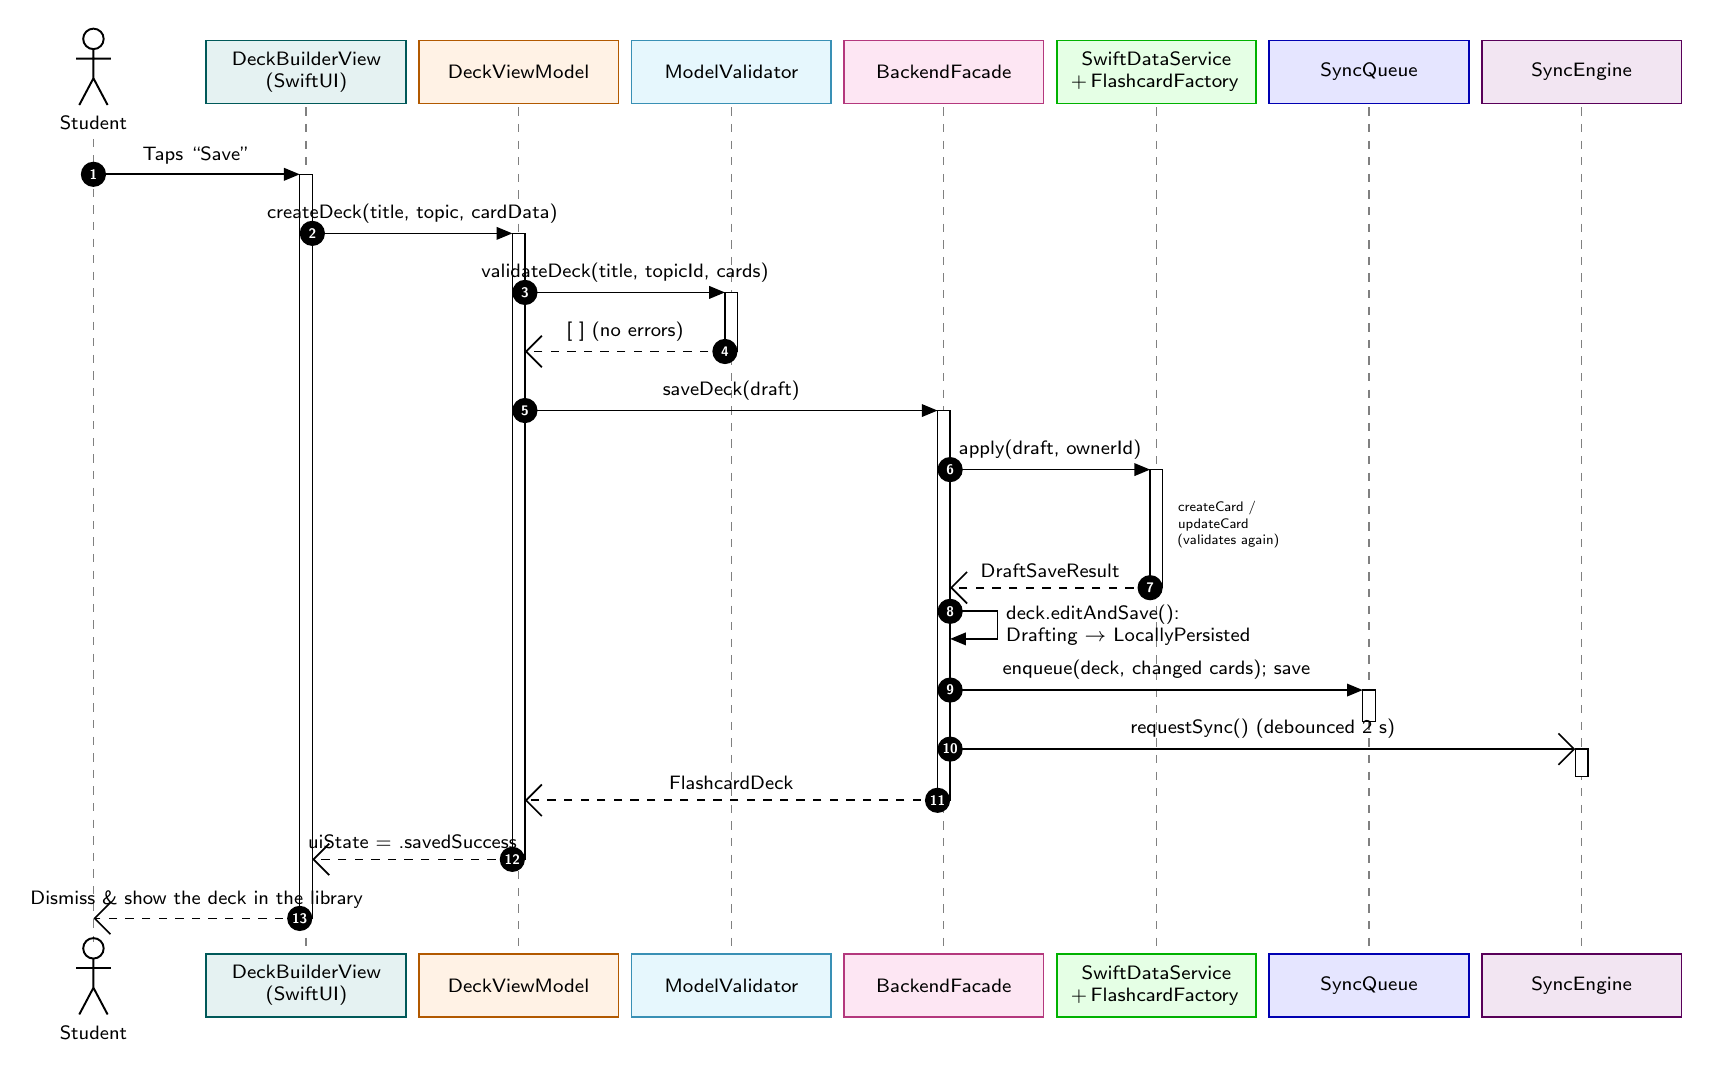
\begin{tikzpicture}[font=\sffamily\scriptsize]
  % Lifeline x-positions
  \def\xS{0}\def\xV{2.7}\def\xM{5.4}\def\xA{8.1}\def\xF{10.8}\def\xD{13.5}\def\xQ{16.2}\def\xE{18.9}
  \def\ytop{0}\def\ybot{-11.6}
  % Heads
  \pic at (\xS,\ytop) {stickman};
  \node at (\xS,\ytop-0.65) {Student};
  \foreach \x/\n/\c in {\xV/{DeckBuilderView\\(SwiftUI)}/teal,
                        \xM/DeckViewModel/orange,
                        \xA/ModelValidator/cyan,
                        \xF/BackendFacade/magenta,
                        \xD/{SwiftDataService\\+\,FlashcardFactory}/green,
                        \xQ/SyncQueue/blue,
                        \xE/SyncEngine/violet}{
    \node[draw=\c!70!black, fill=\c!10, align=center, minimum height=0.8cm,
          text width=2.3cm, line width=0.6pt] at (\x,\ytop) {\n};
    \node[draw=\c!70!black, fill=\c!10, align=center, minimum height=0.8cm,
          text width=2.3cm, line width=0.6pt] at (\x,\ybot) {\n};
    \draw[dashed, gray] (\x,\ytop-0.45) -- (\x,\ybot+0.45);
  }
  \draw[dashed, gray] (\xS,\ytop-0.85) -- (\xS,\ybot+0.55);
  \pic at (\xS,\ybot+0.05) {stickman};
  \node at (\xS,\ybot-0.6) {Student};
  % Activation bars
  \foreach \x/\a/\b in {\xV/-1.3/-10.75, \xM/-2.05/-10.0, \xA/-2.8/-3.55,
                        \xF/-4.3/-9.25, \xD/-5.05/-6.55, \xQ/-7.85/-8.25, \xE/-8.6/-8.95}{
    \fill[white] (\x-0.08,\a) rectangle (\x+0.08,\b);
    \draw[line width=0.5pt] (\x-0.08,\a) rectangle (\x+0.08,\b);
  }
  % Messages: \msg{step}{from x}{to x}{y}{label}{style}
  \newcommand{\msg}[6]{%
    \draw[#6] (#2,#4) -- node[above=2.5pt, inner sep=1pt] {#5} (#3,#4);
    \node[circle, fill=black, text=white, inner sep=0.5pt, minimum size=3.2mm,
          font=\sffamily\tiny\bfseries] at (#2,#4) {#1};}
  % Self message: \self{step}{x}{y}{label}
  \newcommand{\selfmsg}[4]{%
    \draw[sync] (#2+0.08,#3) -- ++(0.6,0) -- ++(0,-0.35) -- (#2+0.08,#3-0.35);
    \node[anchor=west, inner sep=1pt, align=left] at (#2+0.75,#3-0.17) {#4};
    \node[circle, fill=black, text=white, inner sep=0.5pt, minimum size=3.2mm,
          font=\sffamily\tiny\bfseries] at (#2+0.08,#3) {#1};}
  \tikzset{sync/.style={line width=0.6pt, -{Triangle[length=2mm,width=1.6mm]}},
           ret/.style={line width=0.6pt, dashed, -{Straight Barb[length=2mm]}},
           async/.style={line width=0.6pt, -{Straight Barb[length=2mm]}}}
  \msg{1}{\xS}{\xV-0.08}{-1.3}{Taps ``Save''}{sync}
  \msg{2}{\xV+0.08}{\xM-0.08}{-2.05}{createDeck(title, topic, cardData)}{sync}
  \msg{3}{\xM+0.08}{\xA-0.08}{-2.8}{validateDeck(title, topicId, cards)}{sync}
  \msg{4}{\xA-0.08}{\xM+0.08}{-3.55}{[ ] (no errors)}{ret}
  \msg{5}{\xM+0.08}{\xF-0.08}{-4.3}{saveDeck(draft)}{sync}
  \msg{6}{\xF+0.08}{\xD-0.08}{-5.05}{apply(draft, ownerId)}{sync}
  \node[align=left, anchor=west, font=\sffamily\tiny, text width=2.2cm] at (\xD+0.15,-5.75) {createCard /\\updateCard\\(validates again)};
  \msg{7}{\xD-0.08}{\xF+0.08}{-6.55}{DraftSaveResult}{ret}
  \selfmsg{8}{\xF}{-6.85}{deck.editAndSave():\\Drafting $\to$ LocallyPersisted}
  \msg{9}{\xF+0.08}{\xQ-0.08}{-7.85}{enqueue(deck, changed cards); save}{sync}
  \msg{10}{\xF+0.08}{\xE-0.08}{-8.6}{requestSync() (debounced 2 s)}{async}
  \msg{11}{\xF-0.08}{\xM+0.08}{-9.25}{FlashcardDeck}{ret}
  \msg{12}{\xM-0.08}{\xV+0.08}{-10.0}{uiState = .savedSuccess}{ret}
  \msg{13}{\xV-0.08}{\xS}{-10.75}{Dismiss \& show the deck in the library}{ret}
\end{tikzpicture}}
\caption{UML sequence diagram: Create Flashcard Deck via in-app form (UC-01)}
\label{fig:sequence}
\end{figure}

Figure~\ref{fig:sequence} models the main success scenario of UC-01. The student
edits the draft and selects \emph{Save} (1). \texttt{DeckBuilderView} calls
\texttt{DeckViewModel.save()}, which calls \texttt{createDeck(title, topic,
cardData)} for a new deck (2). The view model validates the whole draft with
\texttt{ModelValidator} (3); an empty list of field errors means the draft is valid
(4). The view model then passes the draft to \texttt{BackendFacade.saveDeck()} (5),
the only backend operation it depends on (through the \texttt{DeckBackend} protocol).
The facade asks \texttt{SwiftDataService} to apply the draft (6). It creates or
updates every card through \texttt{FlashcardFactory}, which validates the content a
second time, so no card can bypass the rules. \texttt{SwiftDataService} reports which
cards changed (7). The deck takes the \emph{edit} and \emph{save} transitions of the
State pattern into \emph{LocallyPersisted} (8). The facade queues the deck and its
changed cards, saves the store (9), and asks \texttt{SyncEngine} for a sync two
seconds later (10), so replication runs in the background and rapid saves share one
push. The facade returns the saved deck (11), the view model publishes
\texttt{savedSuccess} (12), and the view dismisses the form (13).

The deck is persisted locally before any network activity (FR-44), which enables
offline deck creation (NFR-08). If validation fails at step 4, the view model stores
the field errors, the view moves to the first invalid card, and the flow stops before
the facade is called (FR-10).

% =====================================================================
\section{UML State Diagram}
% =====================================================================

\begin{figure}[!htbp]
\centering
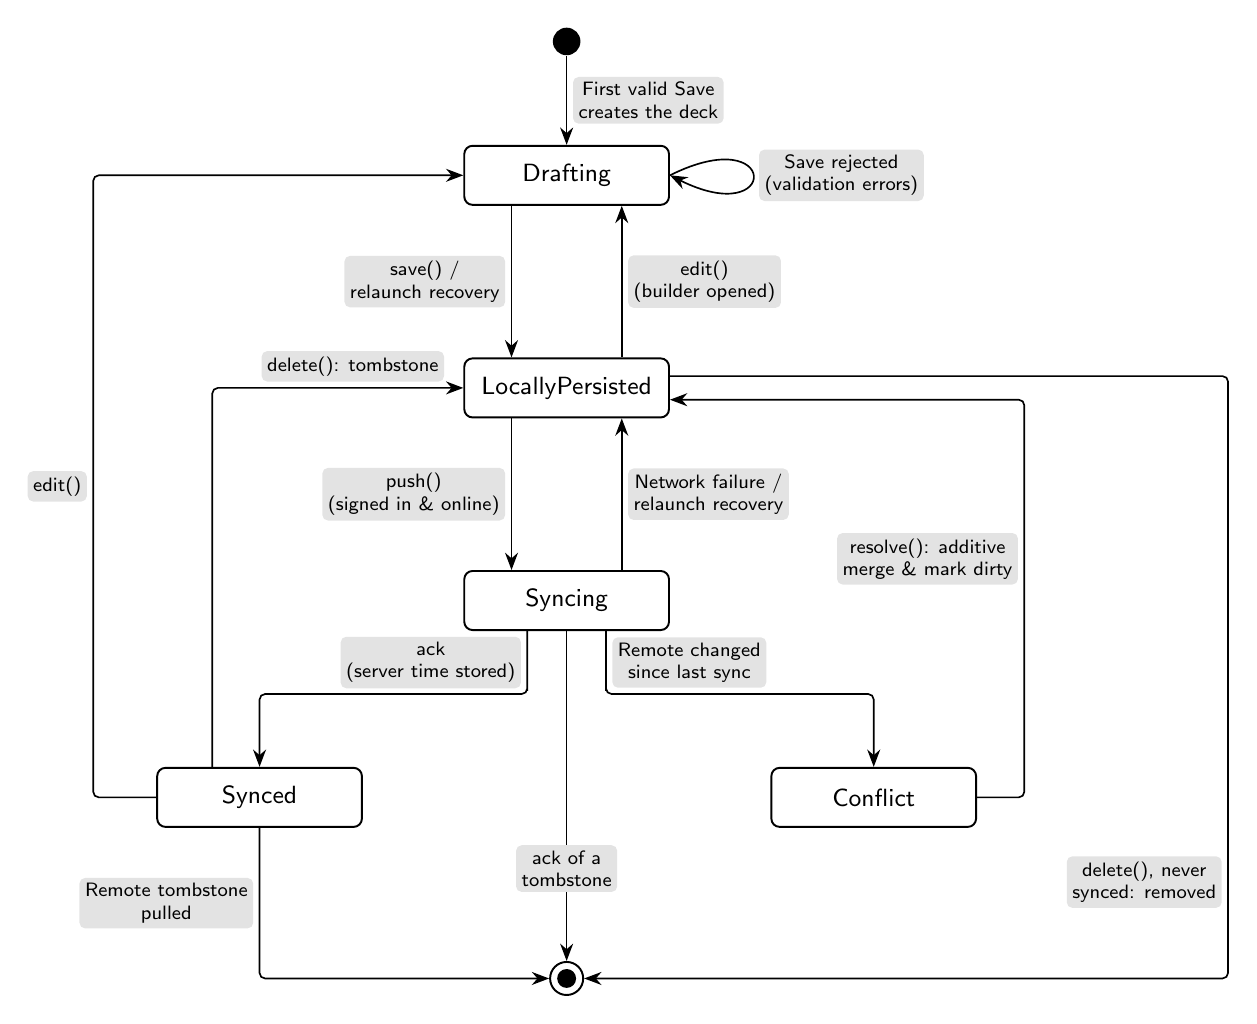
\begin{tikzpicture}[font=\sffamily\scriptsize]
  % States
  \node[circle, fill=black, minimum size=3.5mm, inner sep=0pt] (init) at (0,0) {};
  \node[state] (draft) at (0,-1.7)  {Drafting};
  \node[state] (lp)    at (0,-4.4)  {LocallyPersisted};
  \node[state] (sync)  at (0,-7.1)  {Syncing};
  \node[state] (done)  at (-3.9,-9.6){Synced};
  \node[state] (conf)  at (3.9,-9.6) {Conflict};
  \node[circle, draw, line width=0.7pt, minimum size=4.2mm, inner sep=0pt] (fin) at (0,-11.9) {};
  \node[circle, fill=black, minimum size=2.4mm, inner sep=0pt] at (fin) {};
  % Transitions
  \draw[trans] (init) -- node[glbl, right=2pt] {First valid Save\\creates the deck} (draft);
  \draw[trans] (draft.east) .. controls +(1.4,0.7) and +(1.4,-0.7) ..
        node[glbl, right=2pt] {Save rejected\\(validation errors)} (draft.east);
  \draw[trans] ([xshift=-7mm]draft.south) -- node[glbl, left=2pt] {save() /\\relaunch recovery} ([xshift=-7mm]lp.north);
  \draw[trans] ([xshift=7mm]lp.north) -- node[glbl, right=2pt] {edit()\\(builder opened)} ([xshift=7mm]draft.south);
  \draw[trans] ([xshift=-7mm]lp.south) -- node[glbl, left=2pt] {push()\\(signed in \& online)} ([xshift=-7mm]sync.north);
  \draw[trans] ([xshift=7mm]sync.north) -- node[glbl, right=2pt] {Network failure /\\relaunch recovery} ([xshift=7mm]lp.south);
  \draw[trans] ([xshift=-5mm]sync.south) |- node[glbl, pos=0.25, left=2pt] {ack\\(server time stored)} ++(0,-0.8) -| (done.north);
  \draw[trans] ([xshift=5mm]sync.south)  |- node[glbl, pos=0.25, right=2pt] {Remote changed\\since last sync} ++(0,-0.8) -| (conf.north);
  \draw[trans] (sync.south) -- node[glbl, pos=0.72] {ack of a\\tombstone} (fin.north);
  \draw[trans] (conf.east) -- ++(0.6,0) |- node[glbl, pos=0.3, left=2pt] {resolve(): additive\\merge \& mark dirty} ([yshift=-1.5mm]lp.east);
  \draw[trans] (done.west) -- ++(-0.8,0) |- node[glbl, pos=0.25, left=2pt] {edit()} (draft.west);
  \draw[trans] ([xshift=-6mm]done.north) |- node[glbl, pos=0.78, above=2pt] {delete(): tombstone} (lp.west);
  \draw[trans] ([yshift=1.5mm]lp.east) -- (8.4,-4.25) |- node[glbl, pos=0.42, left=2pt] {delete(), never\\synced: removed} (fin.east);
  \draw[trans] (done.south) |- node[glbl, pos=0.25, left=2pt] {Remote tombstone\\pulled} (fin.west);
\end{tikzpicture}
\caption{UML state diagram: FlashcardDeck sync lifecycle}
\label{fig:state}
\end{figure}

Figure~\ref{fig:state} models the lifecycle of a user-created \texttt{FlashcardDeck}
across five states: \emph{Drafting}, \emph{LocallyPersisted}, \emph{Syncing},
\emph{Synced}, and \emph{Conflict}. The deck model is created by its first valid save;
while a new deck is being written, the builder edits an in-memory draft, so a save that
fails validation leaves no deck behind and an existing deck stays in \emph{Drafting}.

A valid save moves the deck to \emph{LocallyPersisted}. When the student is signed in
and online, \texttt{SyncEngine} pushes it, moving it to \emph{Syncing}. A network
failure returns it to \emph{LocallyPersisted} for a retry with exponential backoff, so
no local changes are lost. A successful acknowledgment stores the server's update
timestamp and moves the deck to \emph{Synced}. If that timestamp has moved past the one
stored at the last sync, another device changed the deck, and it moves to
\emph{Conflict}. There the additive merge runs, and \texttt{resolve()} marks the deck
dirty and returns it to \emph{LocallyPersisted}, from which it is pushed again in the
same sync cycle. Editing a synced deck returns it to \emph{Drafting}.

Two recovery transitions run at app launch, so that a deck is never stranded: a deck
left in \emph{Syncing} by a terminated app returns to \emph{LocallyPersisted}, and so
does a deck persisted in \emph{Drafting}. A deck left in \emph{Conflict} is merged
again on the next push.

A deck may be deleted only from \emph{LocallyPersisted} or \emph{Synced}; deletion is
unavailable in \emph{Drafting}, \emph{Syncing}, and \emph{Conflict}, which prevents
orphaned remote records. A deck that has never synced is removed at once. A deck that
has synced before becomes a tombstone in \emph{LocallyPersisted} (a \emph{Synced} deck
moves there), and a delete operation is queued; the deck is removed when the server
acknowledges the tombstone (FR-12). A tombstone pulled from another device removes a
\emph{Synced} deck. Starter decks (FR-15) never enter this lifecycle: they cannot be
edited, deleted, or pushed, only hidden.

This diagram is the specification for the State pattern (Section~\ref{sec:state}).
Each state is implemented as a type, each transition as the return value of an
\texttt{on\ldots()} method, and each transition and each disallowed operation is
covered by a unit test (risk R9).

% =====================================================================
\section{UML Class Diagrams and Design Patterns}
% =====================================================================
Section~\ref{sec:domain} presents the core domain model, and
Sections~\ref{sec:factory} through~\ref{sec:facade} present one Gang of Four design
pattern from each category. Visibility is denoted by \texttt{+} (public), \texttt{-}
(private), and \texttt{\#} (protected).

\subsection{Core Domain Model}\label{sec:domain}
\begin{figure}[!htbp]
\centering
\begin{tikzpicture}
  \node[cls={orange}{6.0cm}] (vm) at (-3.0,0) {\ctitle{\textbf{DeckViewModel}}
    \nodepart{two}\raggedright +draft: DeckDraft\\ +fieldErrors: [ValidationField: String]\\ +uiState: UIState\\ \priv backend: DeckBackend
    \nodepart{three}\raggedright +createDeck(title, topic, cardData) : FlashcardDeck?\\ +updateDeck() : FlashcardDeck?\\ +save() : FlashcardDeck?\\ +addCard(after: UUID?) : UUID\\ +deleteCard(cardID: UUID)\\ +validateNow() : [FieldError]\\ (also duplicate, restore, move, toggleSnippet)};
  \node[cls={gray}{4.6cm}] (db) at (3.9,0.6) {\ctitle{\st{interface}\\\textbf{DeckBackend}}
    \nodepart{two}~
    \nodepart{three}\raggedright +saveDeck(draft) : FlashcardDeck\\ +deleteDeck(deck)\\ +setHidden(hidden, deck)};
  \node[cls={violet}{4.6cm}, anchor=north] (bf) at (3.9,-1.6) {\ctitle{\textbf{BackendFacade}}\nodepart{two}~\nodepart{three}\raggedright see Fig.~\ref{fig:facade}};
  \node[cls={magenta}{5.6cm}, anchor=north] (deck) at (-3.0,-5.0) {\ctitle{\textbf{FlashcardDeck}}
    \nodepart{two}\raggedright +id: UUID\\ +title: String\\ +topicId: String\\ +origin: DeckOrigin\\ +isHidden: Bool\\ +ownerId: UUID?\\ +syncState: DeckSyncStateKind\\ +deletedAt: Date?
    \nodepart{three}\raggedright +activeCards: [Flashcard] \{get\}\\ +cardCount: Int \{get\}\\ +masteryRate: Double \{get\}\\ \textasciitilde markDirty(at: Date)};
  \node[cls={cyan}{4.6cm}, anchor=north] (sds) at (3.9,-5.0) {\ctitle{\textbf{SwiftDataService}}
    \nodepart{two}\raggedright \priv context: ModelContext\\ \priv factory: FlashcardFactory
    \nodepart{three}\raggedright +apply(draft, ownerId) : DraftSaveResult\\ +fetch(id: UUID) : FlashcardDeck?\\ +fetchCard(id: UUID) : Flashcard?};
  \node[cls={teal}{5.6cm}, anchor=north] (card) at (-3.0,-11.0) {\ctitle{\textbf{Flashcard}}
    \nodepart{two}\raggedright +id: UUID\\ +prompt: String\\ +answer: String\\ +codeSnippet: CodeSnippet?\\ +difficulty: Difficulty?\\ +sortIndex: Int\\ +masteryScore: Int \{readOnly\}\\ +retiredAt: Date?
    \nodepart{three}\raggedright +updateMastery(rating: CardRating)\\ +resetMastery()\\ +toPayload() : FlashcardPayload};
  \node[cls={green}{4.0cm}, anchor=north] (cs) at (3.9,-11.0) {\ctitle{\st{struct}\\\textbf{CodeSnippet}}
    \nodepart{two}\raggedright +language: CodeLanguage\\ +source: String
    \nodepart{three}~};
  \draw[dep] (vm.east |- db.west) -- node[lbl] {\st{use}} (db.west);
  \draw[realize] (bf.north) -- (db.south);
  \draw[dep] (bf.south) -- node[lbl] {\st{use}} (sds.north);
  \draw[dep] (sds.west |- deck.north east) ++(0,-0.6) coordinate (p) (sds.west |- p) -- node[lbl] {\st{create}} (deck.east |- p);
  \draw[compo] (deck.south) -- node[lbl] {contains} (card.north)
        node[pos=0.12, right, font=\sffamily\scriptsize] {1}
        node[pos=0.88, right, font=\sffamily\scriptsize] {0..*};
  \draw[compo] (card.east |- cs.north west) ++(0,-0.5) coordinate (q) (card.east |- q) -- (cs.west |- q)
        node[pos=0.85, above, font=\sffamily\scriptsize] {0..1};
\end{tikzpicture}
\caption{UML class diagram: core domain model}
\label{fig:domain}
\end{figure}

\texttt{FlashcardDeck} owns its \texttt{Flashcard} instances through composition
(1 to 0..*): a card cannot exist without its deck, and deleting a deck deletes its
cards. A card owns at most one \texttt{CodeSnippet}, a value type stored with the card.
\texttt{DeckViewModel} (an \texttt{@Observable} class) edits an in-memory
\texttt{DeckDraft} rather than the stored deck, so an abandoned edit never touches the
store. It depends only on the \texttt{DeckBackend} protocol, which
\texttt{BackendFacade} implements, so its unit tests run against the real facade in
local-only mode with no network. The facade applies a saved draft through
\texttt{SwiftDataService}, which creates and updates cards through
\texttt{FlashcardFactory} (Section~\ref{sec:factory}).

\texttt{FlashcardDeck} stores a \texttt{topicId} that refers to the predefined topic
list, together with its \texttt{origin} (user or starter), \texttt{isHidden},
\texttt{ownerId}, and a \texttt{deletedAt} tombstone for synchronization. Its card
count and mastery rate are computed properties. Cards are attached through the
composition relationship, so no \texttt{addCard()} operation is needed. Validation
lives in \texttt{ModelValidator}, which the factory calls for every card, rather than
in the model classes. A card's payload is a typed \texttt{FlashcardPayload}, and mastery
changes take a \texttt{CardRating}.

% ---------------------------------------------------------------------
\FloatBarrier
\subsection{Creational Pattern: Factory}\label{sec:factory}
\begin{figure}[!htbp]
\centering
\begin{tikzpicture}
  \foreach \x/\n/\name in {-5.4/sds/SwiftDataService, -1.8/sdl/StarterDeckLoader, 1.8/rca/RemoteChangeApplier, 5.4/cr/ConflictResolver}
    \node[cls={magenta}{3.0cm}] (\n) at (\x,0) {\ctitle{\textbf{\name}}\nodepart{two}~\nodepart{three}~};
  \node[cls={orange}{11.4cm}, anchor=north] (ff) at (0,-1.6) {\ctitle{\textbf{FlashcardFactory}}
    \nodepart{two}\raggedright \priv validator: ModelValidator\\ \priv now: () $\to$ Date
    \nodepart{three}\raggedright +createCard(id, prompt, answer, code?, difficulty?, sortIndex) : Flashcard\\ +createCard(from payload: FlashcardPayload) : Flashcard\\ +updateCard(card, prompt, answer, code?, difficulty?, sortIndex) : Bool\\ +applyRemote(payload: FlashcardPayload, to card: Flashcard)\\ \priv validatedSnippet(payload, id) : CodeSnippet?\\ \priv applyDefaults(payload) : FlashcardPayload};
  \node[cls={cyan}{4.4cm}, anchor=north] (fc) at (-2.4,-6.3) {\ctitle{\textbf{Flashcard}}
    \nodepart{two}\raggedright +id: UUID\\ +prompt: String\\ +answer: String\\ +codeSnippet: CodeSnippet?
    \nodepart{three}\raggedright \textasciitilde init(token: Token, \ldots)};
  \node[cls={gray}{3.6cm}, anchor=north] (tk) at (3.6,-6.3) {\ctitle{\textbf{FlashcardFactory.Token}}
    \nodepart{two}~\nodepart{three}\raggedright \priv init() (file-private)};
  \node[cls={green}{3.4cm}, anchor=north] (cs) at (-2.4,-9.4) {\ctitle{\st{struct}\\\textbf{CodeSnippet}}
    \nodepart{two}\raggedright +language: CodeLanguage\\ +source: String
    \nodepart{three}~};
  \foreach \n in {sds,sdl,rca,cr}
    \draw[dep] (\n.south) -- node[lbl] {\st{use}} (\n.south |- ff.north);
  \draw[dep] ([xshift=-2.4cm]ff.south) -- node[lbl] {\st{create}} (fc.north);
  \draw[dep] ([xshift=3.6cm]ff.south) -- node[lbl] {\st{create}} (tk.north);
  \draw[dep] (fc.east |- tk.west) -- node[lbl] {requires} (tk.west);
  \draw[compo] (fc.south) -- (cs.north) node[pos=0.5, right, font=\sffamily\scriptsize] {0..1};
\end{tikzpicture}
\caption{UML class diagram: Factory pattern (creational)}
\label{fig:factory}
\end{figure}

\textbf{Problem.} Flashcards are created or changed in four places: saving the deck
builder's draft, loading the bundled starter decks (FR-14), applying changes pulled
from the server, and merging a sync conflict. All four need identical handling:
normalizing text and code (line endings, indentation, trailing whitespace), applying
defaults, building the optional \texttt{CodeSnippet}, and validating against the card
rules, before a card is saved locally.

\textbf{Solution.} All card creation and content changes go through
\texttt{FlashcardFactory}. When the facade saves a draft,
\texttt{SwiftDataService.apply()} calls \texttt{createCard} and \texttt{updateCard};
\texttt{StarterDeckLoader} calls \texttt{createCard(from:)} and \texttt{updateCard} for
bundled cards; \texttt{RemoteChangeApplier} and \texttt{ConflictResolver} call
\texttt{createCard(from:)} and \texttt{applyRemote} for cards from the server. Each
operation normalizes its input, validates it through the factory's
\texttt{ModelValidator}, and throws field errors that the deck builder shows inline.

\textbf{Consequences.} Because every card is constructed and validated identically,
local, bundled, and remote content remain consistent. The rule that no card is created
outside the factory is enforced by the compiler rather than by code review:
\texttt{Flashcard}'s initializer requires a \texttt{FlashcardFactory.Token}, and only
the factory's source file can create one.

% ---------------------------------------------------------------------
\FloatBarrier
\subsection{Behavioral Pattern: State}\label{sec:state}
\begin{figure}[!htbp]
\centering
\begin{tikzpicture}
  \node[cls={magenta}{6.6cm}] (deck) at (0,0) {\ctitle{\textbf{FlashcardDeck} (context)}
    \nodepart{two}\raggedright \priv syncStateRaw: String (persisted)\\ +currentState: DeckSyncState \{get\}\\ +lastSyncedAt: Date?\\ +serverUpdatedAt: Date?
    \nodepart{three}\raggedright +save()\quad +edit()\quad +push()\quad +resolve()\\ +receive(result: RemoteResult)\\ +delete() : Bool\quad +editAndSave()\\ +recoverAfterLaunch() : Bool\\ +setState(state: DeckSyncState)};
  \node[cls={teal}{7.4cm}, anchor=north] (ds) at (0,-4.3) {\ctitle{\st{interface}\\\textbf{DeckSyncState}}
    \nodepart{two}\raggedright +kind: DeckSyncStateKind\\ +name: String
    \nodepart{three}\raggedright +onSave(deck) : DeckSyncState\\ +onEdit(deck) : DeckSyncState\\ +onPush(deck) : DeckSyncState\\ +onRemoteResponse(deck, result) : DeckSyncState\\ +onResolve(deck) : DeckSyncState\\ +onDelete(deck) : DeckSyncState?\\ (default for every event: no transition, return self)};
  \node[cls={orange}{2.25cm}, anchor=north] (s3) at ([yshift=-1.1cm]ds.south) {\ctitle{\textbf{SyncingState}}\nodepart{two}~\nodepart{three}~};
  \node[cls={cyan}{3.05cm}, left=0.35cm of s3]  (s2) {\ctitle{\textbf{LocallyPersistedState}}\nodepart{two}~\nodepart{three}~};
  \node[cls={orange}{2.25cm}, left=0.35cm of s2] (s1) {\ctitle{\textbf{DraftingState}}\nodepart{two}~\nodepart{three}~};
  \node[cls={violet}{2.25cm}, right=0.35cm of s3] (s4) {\ctitle{\textbf{SyncedState}}\nodepart{two}~\nodepart{three}~};
  \node[cls={red}{2.25cm}, right=0.35cm of s4]    (s5) {\ctitle{\textbf{ConflictState}}\nodepart{two}~\nodepart{three}~};
  \draw[dep] (deck.south) -- node[lbl] {currentState (rebuilt from syncStateRaw)} (ds.north);
  \draw[realize] (s1.north) |- ++(0,0.55) -| ([xshift=-2.6cm]ds.south);
  \draw[realize] (s2.north) |- ++(0,0.35) -| ([xshift=-1.3cm]ds.south);
  \draw[realize] (s3.north) -- (ds.south);
  \draw[realize] (s4.north) |- ++(0,0.35) -| ([xshift=1.3cm]ds.south);
  \draw[realize] (s5.north) |- ++(0,0.55) -| ([xshift=2.6cm]ds.south);
\end{tikzpicture}
\caption{UML class diagram: State pattern (behavioral)}
\label{fig:statepattern}
\end{figure}

\textbf{Problem.} A deck passes through five synchronization states
(Figure~\ref{fig:state}), and the same operation has different effects in each.
Saving a new deck creates it, whereas saving edits to a previously synchronized deck
must mark it dirty so that the local and remote copies can be merged. Implementing
these rules with conditional logic distributed across the codebase risks overwritten,
duplicated, or lost data.

\textbf{Solution.} Each state is a type conforming to the \texttt{DeckSyncState}
protocol, and \texttt{FlashcardDeck} is the context. SwiftData cannot store a protocol
value, so the deck persists only the state's kind (\texttt{syncStateRaw}) and rebuilds
the state object on demand (\texttt{currentState}). Each context operation forwards an
event to the current state, which performs the transition's effects and returns the
next state. A protocol extension supplies the default for every event: no transition,
so the state returns itself. For example, \texttt{SyncingState.onPush()} returns
itself because a push is already in progress. Each state overrides only the events
that have arrows in Figure~\ref{fig:state}; only \texttt{ConflictState} accepts
\texttt{resolve()}, and only \texttt{LocallyPersistedState} and \texttt{SyncedState}
allow \texttt{delete()}. Starter decks ignore every event.

\textbf{Consequences.} Each synchronization rule is defined in exactly one type. The
cost is five small types in place of a single enumeration, which increases the risk
of omitting a transition when a state is added. This risk is mitigated by keeping all
states in \texttt{DeckSyncState.swift} and unit-testing every transition and every
disallowed operation in Figure~\ref{fig:state} (risk R9).

% ---------------------------------------------------------------------
\FloatBarrier
\subsection{Structural Pattern: Fa\c{c}ade}\label{sec:facade}
\begin{figure}[!htbp]
\centering
\resizebox{\textwidth}{!}{%
\begin{tikzpicture}
  \node[cls={orange}{3.6cm}] (vm) at (-5.2,0) {\ctitle{\textbf{DeckViewModel}}
    \nodepart{two}\raggedright \priv backend: DeckBackend
    \nodepart{three}~};
  \node[cls={gray}{3.8cm}] (db) at (0,0) {\ctitle{\st{interface}\\\textbf{DeckBackend}}\nodepart{two}~\nodepart{three}~};
  \node[cls={teal}{3.6cm}] (views) at (5.2,0) {\ctitle{\textbf{SwiftUI views}}
    \nodepart{two}\raggedright (environment object)
    \nodepart{three}~};
  \node[cls={magenta}{7.0cm}, anchor=north] (bf) at (0,-1.7) {\ctitle{\textbf{BackendFacade}}
    \nodepart{two}\raggedright +authState: AuthState\\ +pendingCount: Int\\ +engine: SyncEngine\\ \priv auth: AuthProviding?\\ \priv context: ModelContext\\ \priv cursors: SyncCursorStore
    \nodepart{three}\raggedright +signInWithGoogle()\qquad +signOut(removingLocalDecks: Bool)\\ +saveDeck(draft: DeckDraft) : FlashcardDeck\\ +deleteDeck(deck)\qquad +deleteCard(card)\qquad +setHidden(hidden, deck)\\ +syncPending()\qquad +didResetProgress()\\ +start()\qquad +handle(url: URL) : Bool};
  \node[cls={orange}{4.1cm}, anchor=north] (a) at (-6.4,-8.2) {\ctitle{\textbf{SupabaseAuthProvider}\\\st{AuthProviding}}
    \nodepart{two}~\nodepart{three}\raggedright +signIn(presenting:) : AppUser?\\ +signOut()\\ +authStateStream()};
  \node[cls={violet}{4.1cm}, anchor=north] (e) at (-1.9,-8.2) {\ctitle{\textbf{SyncEngine}}
    \nodepart{two}\raggedright \priv remote: RemoteDeckStore?\\ \priv reachability: Reachability
    \nodepart{three}\raggedright +syncNow() : Bool\\ +requestSync(after:)\\ +start()\qquad +stop()};
  \node[cls={green}{4.1cm}, anchor=north] (l) at (2.6,-8.2) {\ctitle{\textbf{SwiftDataService}, \textbf{SyncQueue}}
    \nodepart{two}~\nodepart{three}\raggedright created per call on the\\ facade's ModelContext};
  \node[cls={cyan}{4.6cm}, anchor=north] (r) at (-4.3,-11.8) {\ctitle{\textbf{SupabaseDataClient}\\\st{RemoteDeckStore}}
    \nodepart{two}~\nodepart{three}\raggedright +upsertDecks(\_:)\qquad +upsertCards(\_:)\\ +fetchChanges(since:)\\ +fetchDeckVersions(ids:)\\ +fetchDeckSnapshot(id:)\\ +fetchProfile()\qquad +upsertProfile(\_:)\\ +appendSyncLog(\_:)};
  \node[cls={violet}{3.4cm}, anchor=north] (n) at (0.5,-11.8) {\ctitle{\textbf{NetworkMonitor}\\\st{Reachability}}
    \nodepart{two}\raggedright +isReachable: Bool
    \nodepart{three}\raggedright +changes()};
  \draw[dep] (vm.east) -- node[lbl] {\st{use}} (db.west);
  \draw[realize] (bf.north -| db.south) -- (db.south);
  \draw[dep] (views.south) |- node[lbl, pos=0.25] {\st{use}} ([yshift=-0.6cm]bf.north east);
  \draw[assoc] ([xshift=-2.6cm]bf.south) |- ++(0,-0.5) -| (a.north);
  \draw[assoc] ([xshift=-1.0cm]bf.south) |- ++(0,-0.75) -| (e.north);
  \draw[dep] ([xshift=2.0cm]bf.south)  |- node[lbl, pos=0.75] {\st{create}} ++(0,-0.75) -| (l.north);
  \draw[assoc] ([xshift=-0.9cm]e.south) |- ++(0,-0.5) -| (r.north);
  \draw[assoc] ([xshift=0.9cm]e.south)  |- ++(0,-0.5) -| (n.north);
  \begin{scope}[on background layer]
    \node[draw=gray, dashed, rounded corners=3pt, fit=(a)(e)(l)(r)(n), inner xsep=0.25cm, inner ysep=0.3cm] (wrap) {};
    \node[anchor=north east, font=\sffamily\scriptsize\itshape, text=gray!40!black] at (wrap.south east) {wrapped backend subsystem};
  \end{scope}
\end{tikzpicture}}
\caption{UML class diagram: Fa\c{c}ade pattern (structural)}
\label{fig:facade}
\end{figure}

\textbf{Problem.} Saving and synchronizing a deck involves several subsystems: the
Google Sign-In SDK, Supabase Auth for session tokens, the PostgREST data API, the
Keychain for the stored session, SwiftData for local storage, the sync queue, and a
reachability check before any network request. If screens and view models invoked these
subsystems directly, every screen would depend on the call order, token handling, and
offline behavior. The user interface would be coupled to Supabase and could not be
tested without a live backend.

\textbf{Solution.} \texttt{BackendFacade} is the single entry point to the backend
subsystem. \texttt{DeckViewModel} depends only on the facade's \texttt{DeckBackend}
protocol (save, delete, hide). Screens reach the facade as a SwiftUI environment object
for sign-in, sign-out, manual sync, and sync status. Internally, the facade saves
locally through \texttt{SwiftDataService}, queues changes in \texttt{SyncQueue}, and
hands synchronization to \texttt{SyncEngine}, which checks connectivity through
\texttt{NetworkMonitor} and pushes and pulls through \texttt{SupabaseDataClient}. The
Supabase and Google types sit behind the \texttt{AuthProviding} and
\texttt{RemoteDeckStore} protocols, and only the \texttt{Services/\allowbreak Backend/\allowbreak Supabase/}
folder imports them (checked by \texttt{check-imports.sh}). Session tokens, endpoint
URLs, and PostgREST responses are not exposed to the user interface. Screens read decks
directly from the local store with SwiftData queries, so the facade needs no fetch
operation.

\textbf{Consequences.} The user interface depends on one class rather than on each
subsystem, the backend provider can be replaced by changing only the adapter folder
(risk R7), and nothing is tested against a live backend: the view models run against
the facade in local-only mode, and the sync engine against mock implementations of the
protocols. The facade may accumulate unrelated backend
responsibilities and become a god class (risk R8). To prevent this, it is limited to
coordination; it is 291 lines long and will be split into \texttt{AuthFacade} and
\texttt{DeckFacade} if it exceeds 300 lines.

% =====================================================================
\section{UML Component Diagram}\label{sec:component}
% =====================================================================

\begin{figure}[!htbp]
\centering
\resizebox{\textwidth}{!}{%
\begin{tikzpicture}[font=\sffamily\scriptsize]
  \tikzset{wcomp/.style={comp, text width=3.6cm},
           ilbl/.style={font=\sffamily\scriptsize\itshape, inner sep=1.5pt}}
  % ---- Client subsystem
  \node[wcomp] (pres)  at (-5.8,0)    {\st{component}\\\textbf{Presentation}\\SwiftUI views and view models};
  \node[wcomp] (back)  at (0,0)       {\st{component}\\\textbf{Backend \& Sync}\\BackendFacade, SyncEngine, SyncQueue, ConflictResolver, DeckSyncState};
  \node[wcomp] (adapt) at (6.4,0)     {\st{component}\\\textbf{Supabase Adapter}\\SupabaseAuthProvider, SupabaseDataClient, KeychainSessionStorage, Google Sign-In SDK};
  \node[wcomp] (local) at (-5.8,-3.3) {\st{component}\\\textbf{Local Store}\\SwiftData container, SwiftDataService, FlashcardFactory};
  \node[wcomp] (net)   at (0,-3.3)    {\st{component}\\\textbf{Network Monitor}\\NetworkMonitor (NWPathMonitor)};
  % Provided interfaces (balls) and their providers
  \node[ball] (iDB)   at (-2.9,0)     {}; \node[ilbl, above=2pt of iDB] {DeckBackend};
  \node[ball] (iMC)   at (-5.8,-1.65) {}; \node[ilbl, left=3pt of iMC] {ModelContext};
  \node[ball] (iRe)   at (0,-1.65)    {}; \node[ilbl, right=3pt of iRe] {Reachability};
  \node[ball] (iAP)   at (3.2,0.35)   {}; \node[ilbl, above=2pt of iAP] {AuthProviding};
  \node[ball] (iRDS)  at (3.2,-0.35)  {}; \node[ilbl, below=2pt of iRDS] {RemoteDeckStore};
  \draw[line width=0.6pt] (back.west) -- (iDB);
  \draw[line width=0.6pt] (local.north) -- (iMC);
  \draw[line width=0.6pt] (net.north) -- (iRe);
  \draw[line width=0.6pt] (adapt.west |- iAP) -- (iAP);
  \draw[line width=0.6pt] (adapt.west |- iRDS) -- (iRDS);
  % Required interfaces (sockets)
  \sock{iDB}{180} \draw[line width=0.6pt] (pres.east) -- ([shift={(180:0.24)}]iDB.center);
  \sock{iMC}{90}  \draw[line width=0.6pt] (pres.south) -- ([shift={(90:0.24)}]iMC.center);
  \sock{iMC}{0}   \draw[line width=0.6pt] ([xshift=-1.2cm]back.south) |- ([shift={(0:0.24)}]iMC.center);
  \sock{iRe}{90}  \draw[line width=0.6pt] (back.south) -- ([shift={(90:0.24)}]iRe.center);
  \sock{iAP}{0}   \draw[line width=0.6pt] (back.east |- iAP) -- ([shift={(0:0.24)}]iAP.center);
  \sock{iRDS}{0}  \draw[line width=0.6pt] (back.east |- iRDS) -- ([shift={(0:0.24)}]iRDS.center);
  \node[anchor=south west, font=\sffamily\scriptsize\bfseries] (t1) at (-7.8,1.0) {\st{subsystem} Client App (iOS)};
  \begin{scope}[on background layer]
    \node[draw=magenta!60!black, fill=magenta!5, line width=0.6pt, inner xsep=0.3cm, inner ysep=0.3cm,
          fit=(t1)(pres)(back)(adapt)(local)(net)] (cf) {};
  \end{scope}
  \foreach \n in {pres,back,adapt,local,net}{\compicon{\n}}

  % ---- Remote
  \node[wcomp] (google) at (-1.0,-7.9) {\st{component}\\\textbf{Google Identity}\\OAuth 2.0 / OpenID Connect};
  \node[wcomp] (gotrue) at (3.6,-7.9)  {\st{component}\\\textbf{Supabase Auth}\\(GoTrue)};
  \node[wcomp] (rest)   at (8.0,-7.9)  {\st{component}\\\textbf{PostgREST}\\enforces RLS policies};
  \node[wcomp] (db)     at (6.3,-11.1) {\st{component}\\\textbf{PostgreSQL}\\profiles, decks, flashcards, sync\_log};
  \node[ball] (iOIDC) at (-1.0,-5.9) {}; \node[ilbl, left=3pt of iOIDC] {OIDC (HTTPS)};
  \node[ball] (iAuth) at (3.6,-5.9)  {}; \node[ilbl, right=3pt of iAuth] {Auth API (HTTPS)};
  \node[ball] (iRest) at (8.0,-5.9)  {}; \node[ilbl, right=3pt of iRest] {REST API (HTTPS)};
  \node[ball] (iSQL)  at (6.3,-9.5)  {}; \node[ilbl, below right=1pt and 3pt of iSQL] {SQL};
  \draw[line width=0.6pt] (google.north) -- (iOIDC);
  \draw[line width=0.6pt] (gotrue.north) -- (iAuth);
  \draw[line width=0.6pt] (rest.north) -- (iRest);
  \draw[line width=0.6pt] (db.north) -- (iSQL);
  \sock{iOIDC}{90} \draw[line width=0.6pt] ([xshift=-1.2cm]adapt.south) |- ++(0,-3.9) -| ([shift={(90:0.24)}]iOIDC.center);
  \sock{iAuth}{90} \draw[line width=0.6pt] (adapt.south) |- ++(0,-4.3) -| ([shift={(90:0.24)}]iAuth.center);
  \sock{iRest}{90} \draw[line width=0.6pt] ([xshift=1.2cm]adapt.south) |- ++(0,-4.3) -| ([shift={(90:0.24)}]iRest.center);
  \sock{iOIDC}{0}  \draw[line width=0.6pt] (gotrue.west) -- ++(-0.5,0) |- ([shift={(0:0.24)}]iOIDC.center);
  \sock{iSQL}{0}   \draw[line width=0.6pt] (rest.south) |- ([shift={(0:0.24)}]iSQL.center);
  \sock{iSQL}{180} \draw[line width=0.6pt] (gotrue.south) |- ([shift={(180:0.24)}]iSQL.center);
  \node[anchor=north west, align=left, font=\sffamily\scriptsize\bfseries] (t2) at (1.75,-10.0) {\st{subsystem}\\Remote Backend\\(Supabase)};
  \begin{scope}[on background layer]
    \node[draw=teal!60!black, fill=teal!5, line width=0.6pt, inner xsep=0.3cm, inner ysep=0.3cm,
          fit=(t2)(gotrue)(rest)(db)] (bf) {};
  \end{scope}
  \foreach \n in {google,gotrue,rest,db}{\compicon{\n}}
\end{tikzpicture}}
\caption{UML component diagram: client and backend subsystems with interfaces}
\label{fig:component}
\end{figure}

Figure~\ref{fig:component} shows the client and backend subsystems and the interfaces
between them in UML 2 ball-and-socket notation: a ball is an interface the component
provides, and a socket is an interface it requires. Each client interface is a protocol
or framework type in the code, so the diagram matches the implementation.

\textbf{Client subsystem.} The \emph{Presentation} component (SwiftUI views and their
view models) requires \texttt{DeckBackend}, the protocol through which the deck builder
saves, deletes, and hides decks, and reads the local store directly through SwiftData's
\texttt{ModelContext}. The \emph{Backend \& Sync} component provides
\texttt{DeckBackend} through \texttt{BackendFacade} and contains the sync queue, the
sync engine, the conflict resolver, and the deck state machine. It requires the local
store, \texttt{Reachability} from the \emph{Network Monitor}, and the two backend
protocols \texttt{AuthProviding} and \texttt{RemoteDeckStore}. The \emph{Supabase
Adapter} provides those two protocols; it is the only component that imports the
Supabase and Google Sign-In libraries (checked by \texttt{check-imports.sh}, risk R7),
and it stores the session in the iOS Keychain. Unit tests replace the adapter and the
network monitor with in-memory mocks, so the whole client is tested without a network.

\textbf{Backend subsystem.} The adapter requires three HTTPS interfaces: Google's OpenID
Connect endpoints, which return the ID token at sign-in; the \emph{Supabase Auth}
(GoTrue) API, which exchanges that token for a session; and the \emph{PostgREST} API for
decks, cards, the profile, and the sync ledger. Supabase Auth also requires Google's
OpenID Connect interface to verify the token. PostgREST and Supabase Auth require SQL
access to \emph{PostgreSQL}, and PostgREST evaluates the Row Level Security policies on
every request. Table~\ref{tab:interfaces} lists every interface.

\begin{table}[H]
\centering
\caption{Component interfaces}
\label{tab:interfaces}
\begin{tabularx}{\textwidth}{@{}L{2.8cm} Y Y@{}}
\toprule
\textbf{Component} & \textbf{Provided Interfaces} & \textbf{Required Interfaces} \\
\midrule
Presentation & -- & \texttt{DeckBackend}: save, delete, and hide decks; \texttt{ModelContext}: read decks, topics, and progress through SwiftData queries \\
Backend \& Sync & \texttt{DeckBackend} (implemented by \texttt{BackendFacade}) & \texttt{ModelContext}; \texttt{Reachability}: connectivity changes; \texttt{AuthProviding}: sign-in and session state; \texttt{RemoteDeckStore}: batched upserts, change pulls, profile, sync ledger \\
Local Store & \texttt{ModelContext}: the versioned SwiftData store (file-protected) & -- \\
Network Monitor & \texttt{Reachability} & -- \\
Supabase Adapter & \texttt{AuthProviding} (\texttt{SupabaseAuthProvider}); \texttt{RemoteDeckStore} (\texttt{SupabaseDataClient}) & OIDC; Auth API; REST API (all HTTPS, TLS 1.3); iOS Keychain (session storage) \\
Google Identity & OIDC: Google sign-in and ID-token verification & -- \\
Supabase Auth & Auth API: exchanges a Google ID token for a session, refreshes it & OIDC; SQL \\
PostgREST & REST API: \texttt{profiles}, \texttt{decks}, \texttt{flashcards}, \texttt{sync\_log} & SQL (each request runs under the caller's RLS policies) \\
PostgreSQL & SQL & -- \\
\bottomrule
\end{tabularx}
\end{table}

% =====================================================================
\section{UML Deployment Diagram}\label{sec:deploy}
% =====================================================================

\begin{figure}[!htbp]
\centering
\resizebox{\textwidth}{!}{%
\begin{tikzpicture}[font=\sffamily\scriptsize]
  % ---- Client node
  \node[artifact, text width=3.0cm] (app) at (0,0) {\st{artifact}\\\textbf{Codey.app}\\(SwiftUI, view models, Google Sign-In and Supabase SDKs)};
  \node[artifact, text width=2.9cm] (sq)  at (-2.3,-2.6) {\st{database}\\SwiftData SQLite store\\(complete unless open)};
  \node[artifact] (kc)  at (2.3,-2.6)  {\st{artifact}\\iOS Keychain\\(Supabase session, this device only)};
  \draw[dep] ([xshift=-0.5cm]app.south) -- node[lbl, left=2pt] {local disk I/O} (sq.north);
  \draw[dep] ([xshift=0.5cm]app.south) -- node[lbl, right=2pt] {Security framework} (kc.north);
  \node[anchor=south, font=\sffamily\scriptsize\bfseries, align=center] (t1) at (0,0.9)
       {\st{device}\\Client Node: Apple iPhone / iOS Simulator (iOS 26+)};
  \begin{scope}[on background layer]
    \node[draw, line width=0.6pt, fill=magenta!6, inner sep=0.3cm, fit=(t1)(app)(sq)(kc)] (n1) {};
    \nodebox{n1}{magenta}
  \end{scope}

  % ---- Google node
  \node[artifact] (oidc) at (8.2,-7.2) {\st{service}\\Google OAuth 2.0 /\\OpenID Connect};
  \node[anchor=south, font=\sffamily\scriptsize\bfseries, align=center] (tg) at (8.2,-6.4)
       {\st{execution environment}\\Google Identity Platform};
  \begin{scope}[on background layer]
    \node[draw, line width=0.6pt, fill=yellow!8, inner sep=0.3cm, fit=(tg)(oidc)] (ng) {};
    \nodebox{ng}{yellow}
  \end{scope}

  % ---- Cloud node
  \node[artifact] (gt) at (-2.1,-7.3) {\st{service}\\GoTrue Auth Service};
  \node[artifact] (pr) at (2.1,-7.3)  {\st{service}\\PostgREST API Engine};
  \node[artifact] (rls) at (2.1,-9.4) {\st{service}\\Row Level Security (RLS) Filter};
  \draw[dep] (pr.south) -- node[lbl] {validates policy} (rls.north);
  \node[anchor=south, font=\sffamily\scriptsize\bfseries, align=center] (t2) at (0,-6.45)
       {\st{execution environment}\\Cloud Node: Supabase Platform (AWS container)};
  \begin{scope}[on background layer]
    \node[draw, line width=0.6pt, fill=teal!6, inner sep=0.3cm, fit=(t2)(gt)(pr)(rls)] (n2) {};
    \nodebox{n2}{teal}
  \end{scope}

  % ---- Data tier node
  \node[artifact, text width=2.2cm] (d0) at (-5.6,-13.4) {\st{table}\\Profiles};
  \node[artifact, text width=2.2cm] (d1) at (-2.8,-13.4) {\st{table}\\Flashcards};
  \node[artifact, text width=2.2cm] (d2) at (0,-13.4)    {\st{database}\\PostgreSQL Relational DB};
  \node[artifact, text width=2.2cm] (d3) at (2.8,-13.4)  {\st{table}\\Decks};
  \node[artifact, text width=2.2cm] (d4) at (5.6,-13.4)  {\st{table}\\Sync Ledger (sync\_log)};
  \node[anchor=south, font=\sffamily\scriptsize\bfseries, align=center] (t3) at (0,-12.6)
       {\st{node}\\Data Tier Node: Managed PostgreSQL Instance};
  \begin{scope}[on background layer]
    \node[draw, line width=0.6pt, fill=orange!6, inner sep=0.3cm, fit=(t3)(d0)(d1)(d2)(d3)(d4)] (n3) {};
    \nodebox{n3}{orange}
  \end{scope}

  % ---- Communication paths
  \draw[line width=0.8pt, -{Stealth[length=2.2mm]}] (n2.north |- n1.south) -- node[glbl] {\st{HTTPS / TLS 1.3}\\port 443} (n2.north);
  \draw[line width=0.8pt, -{Stealth[length=2.2mm]}] ([xshift=0.35cm]n1.east) -| node[glbl, pos=0.75] {\st{HTTPS}\\port 443} (ng.north);
  \draw[line width=0.8pt, -{Stealth[length=2.2mm]}] ([xshift=0.35cm]n2.east |- oidc.west) -- node[glbl, above=1pt] {\st{HTTPS}} (ng.west |- oidc.west);
  \draw[line width=0.8pt, -{Stealth[length=2.2mm]}] (n2.south) -- node[glbl] {\st{TCP / SSL}\\port 5432} (n3.north);
\end{tikzpicture}}
\caption{UML deployment diagram: client, cloud, identity provider, and data tier nodes}
\label{fig:deploy}
\end{figure}

Figure~\ref{fig:deploy} shows the four nodes on which Codey is deployed and the
artifacts each node hosts.
\begin{itemize}
  \item \textbf{Client node} (\st{device}): an iPhone or the iOS Simulator running
        iOS 26 or later. It hosts the \texttt{Codey.app} bundle (including the Google
        Sign-In and Supabase client libraries), the SwiftData SQLite store that
        supports offline use, and the iOS Keychain item that holds the Supabase
        session (FR-02). The store is encrypted with \emph{complete unless open} file
        protection, and the Keychain item is \emph{after first unlock, this device
        only}, so it is never included in a backup (NFR-04).
  \item \textbf{Identity provider node} (\st{execution environment}): Google's OAuth
        2.0 and OpenID Connect service. The app's Google Sign-In sheet obtains an ID
        token from it, and Supabase Auth verifies that token's signature against it.
  \item \textbf{Cloud node} (\st{execution environment}): the Supabase platform,
        running in AWS-hosted containers. It hosts the GoTrue authentication service
        and the PostgREST API engine. Every PostgREST request passes through the Row
        Level Security filter before reaching data (NFR-07).
  \item \textbf{Data tier node}: a managed PostgreSQL instance hosting the
        \texttt{profiles}, \texttt{decks}, and \texttt{flashcards} tables and the
        \texttt{sync\_log} ledger used to audit synchronization. Stored data is
        encrypted at rest (NFR-05). The Free plan includes no automated backups, so
        the team exports the database with \texttt{pg\_dump}
        (\texttt{scripts/backup.sh}) before schema changes (risk R11).
\end{itemize}

\textbf{Communication paths.} Components on the client communicate through in-process
calls and, for the Keychain, through the Security framework. The client communicates
with the cloud node only over HTTPS, and its URL session refuses any protocol below
TLS 1.3 (NFR-06); it reaches Google over HTTPS during sign-in. The cloud node
connects to PostgreSQL over an encrypted TCP/SSL connection on port 5432, which is not
exposed to the client. Database credentials therefore remain within Supabase, and the
client only ever holds the public anon key and the signed-in user's session.

\vfill
\begin{center}
\small\itshape We used AI to help create this document.
\end{center}

\end{document}
